\documentclass[10pt,conference]{IEEEtran}
\IEEEoverridecommandlockouts

\usepackage{cite}
\usepackage{amsmath,amssymb,amsfonts,amsthm}
\usepackage{algorithm}
\usepackage{algorithmic}
\usepackage{graphicx}
\usepackage{textcomp}
\usepackage{xcolor}
\usepackage{booktabs}
\usepackage{microtype}
\usepackage[hidelinks]{hyperref}
\usepackage{tikz}
\usepackage{pgfplots}
\pgfplotsset{compat=1.18}
\usepgfplotslibrary{groupplots}
\usetikzlibrary{arrows.meta,positioning,fit,backgrounds,shapes.geometric,calc}

% Colorblind-safe Okabe-Ito-inspired palette for publication-grade vector figures
\definecolor{ssmqBlue}{HTML}{0072B2}
\definecolor{ssmqOrange}{HTML}{E69F00}
\definecolor{ssmqTeal}{HTML}{009E73}
\definecolor{ssmqPurple}{HTML}{CC79A7}
\definecolor{ssmqRed}{HTML}{D55E00}
\definecolor{ssmqGray}{HTML}{6C757D}

\newtheorem{proposition}{Proposition}

\newcommand{\TraceCount}{600}
\newcommand{\NomSsmqP}{728.5}
\newcommand{\NomNoConeP}{623.3}
\newcommand{\NomFifoP}{524.4}
\newcommand{\NomFifoRetryP}{607.1}
\newcommand{\NomSingP}{862.1}
\newcommand{\NomTreeP}{331.1}
\newcommand{\NomSsmqWidth}{1.32}
\newcommand{\NomNoConeWidth}{2.02}
\newcommand{\NomFifoRetryWidth}{3.11}
\newcommand{\NomSsmqFrr}{5.62}
\newcommand{\NomNoConeFrr}{4.01}
\newcommand{\NomFifoFrr}{9.48}
\newcommand{\NomTreeFrr}{2.48}
\newcommand{\NomSsmqCi}{76.6}
\newcommand{\NomTreeCi}{45.9}
\newcommand{\NomSsmqInv}{70.9}
\newcommand{\NomVsNoCone}{105.2}
\newcommand{\NomVsNoConeLo}{89.7}
\newcommand{\NomVsNoConeHi}{121.1}
\newcommand{\NomVsFifo}{204.0}
\newcommand{\NomVsFifoLo}{187.0}
\newcommand{\NomVsFifoHi}{220.7}
\newcommand{\NomVsFifoR}{121.4}
\newcommand{\NomVsFifoRLo}{99.0}
\newcommand{\NomVsFifoRHi}{142.9}
\newcommand{\NomVsSingGain}{133.6}
\newcommand{\NomVsSingLo}{121.0}
\newcommand{\NomVsSingHi}{146.7}
\newcommand{\NomVsDisj}{+6.6}
\newcommand{\NomVsDisjLo}{-13.1}
\newcommand{\NomVsDisjHi}{+26.0}
\newcommand{\NomVsTree}{397.4}
\newcommand{\NomVsTreeLo}{383.4}
\newcommand{\NomVsTreeHi}{411.0}
\newcommand{\SatSsmqP}{876.6}
\newcommand{\SatNoConeP}{766.4}
\newcommand{\SatFifoRetryP}{777.6}
\newcommand{\SatSingP}{1041.7}
\newcommand{\SatTreeP}{497.8}
\newcommand{\SatVsNoCone}{110.2}
\newcommand{\SatVsNoConeLo}{95.4}
\newcommand{\SatVsNoConeHi}{124.4}
\newcommand{\SatVsFifoR}{99.0}
\newcommand{\SatVsFifoRLo}{80.1}
\newcommand{\SatVsFifoRHi}{117.8}
\newcommand{\SatVsTree}{378.7}
\newcommand{\SatVsTreeLo}{363.9}
\newcommand{\SatVsTreeHi}{393.5}
\newcommand{\DirVsNoCone}{307.8}
\newcommand{\DirVsNoConeLo}{289.0}
\newcommand{\DirVsNoConeHi}{327.1}
\newcommand{\DirVsNoGraph}{405.3}
\newcommand{\DirVsNoGraphLo}{384.0}
\newcommand{\DirVsNoGraphHi}{427.6}
\newcommand{\GitDisjAstTests}{220}
\newcommand{\GitDisjFileTests}{222}
\newcommand{\GitDisjBisectTests}{260}
\newcommand{\GitFifoAstTests}{228}
\newcommand{\GitFifoFileTests}{236}
\newcommand{\GitFifoBisectTests}{266}
\newcommand{\StalePairsN}{6}
\newcommand{\StaleUnsafeEscapes}{6}
\newcommand{\StaleRecheckCatches}{6}
\newcommand{\BlameTotalN}{86}
\newcommand{\BlameAstLoo}{98.8}
\newcommand{\BlameFileLoo}{87.2}
\newcommand{\BlameAstSib}{95.5}
\newcommand{\BlameFileSib}{50.0}
\newcommand{\QuixSiblingN}{12}
\newcommand{\QuixSiblingAst}{12}
\newcommand{\QuixSiblingFile}{6}
\newcommand{\QuixSiblingBlind}{6}
\newcommand{\QuixSameN}{12}
\newcommand{\QuixSameAst}{6}
\newcommand{\QuixSameFile}{6}
\newcommand{\QuixDoubleN}{12}
\newcommand{\QuixDoubleAst}{0}

% AUTO-GENERATED BY eval/export_v8_displays.py -- DO NOT EDIT
\newcommand{\ObsDays}{8}
\newcommand{\ObsDistinctPrs}{83}
\newcommand{\ObsAdmissions}{100}
\newcommand{\ObsEvictions}{17}
\newcommand{\ObsMultiPrs}{12}
\newcommand{\ObsTsEnum}{431}
\newcommand{\ObsTsFetched}{246}
\newcommand{\ObsTsNotFound}{164}
\newcommand{\ObsTsDrafts}{21}
\newcommand{\ObsTsPrs}{43}
\newcommand{\ObsTsAdmissions}{44}
\newcommand{\ObsTsFailedChecks}{1}
\newcommand{\ObsTsSojournP}{17.1}
\newcommand{\ObsTsSojournPnf}{21.3}
\newcommand{\ObsCargoEnum}{243}
\newcommand{\ObsCargoFetched}{161}
\newcommand{\ObsCargoNotFound}{71}
\newcommand{\ObsCargoDrafts}{11}
\newcommand{\ObsCargoPrs}{40}
\newcommand{\ObsCargoAdmissions}{56}
\newcommand{\ObsCargoEvictions}{16}
\newcommand{\ObsCargoFailedChecks}{13}
\newcommand{\ObsCargoConflicts}{2}
\newcommand{\ObsCargoTimeouts}{1}
\newcommand{\ObsCargoMultiPrs}{11}
\newcommand{\ObsCargoSojournP}{34.2}
\newcommand{\ObsCargoSojournPnf}{39.2}
\newcommand{\ObsCargoDiscordant}{114}
\newcommand{\ObsTsWfScanned}{690}
\newcommand{\ObsTsWfSelected}{45}
\newcommand{\ObsTsWfCaveats}{8}
\newcommand{\ObsTsWfDiscordant}{45}
\newcommand{\ObsTsWfP}{16.0}
\newcommand{\ObsTsWfMean}{16.1}
\newcommand{\ObsTsWfPnf}{18.8}
\newcommand{\UnfDensity}{73.3}
\newcommand{\FcDensity}{10.8}
\newcommand{\DirTargetDensity}{46.7}
\newcommand{\FcNomWidth}{1.89}
\newcommand{\FcNomP}{607.7}
\newcommand{\FcNomFrr}{4.82}
\newcommand{\FcNomAcc}{105.0}
\newcommand{\FcNomCi}{66.6}
\newcommand{\FcNomStale}{368.2}
\newcommand{\FcNomRec}{0.11}
\newcommand{\FcDirRec}{0.54}
\newcommand{\FcNomDeltaP}{-15.6}
\newcommand{\FcNomDeltaPLo}{-30.5}
\newcommand{\FcNomDeltaPHi}{-0.5}
\newcommand{\FcNomSignP}{0.115}
\newcommand{\FcNomDeltaFrr}{+0.82}
\newcommand{\FcNomDeltaFrrLo}{+0.29}
\newcommand{\FcNomDeltaFrrHi}{+1.42}
\newcommand{\FcNomDeltaAcc}{-0.95}
\newcommand{\FcNomGainVsUnf}{120.8}
\newcommand{\FcSatP}{770.5}
\newcommand{\FcSatFrr}{3.89}
\newcommand{\FcSatDeltaP}{+4.1}
\newcommand{\FcSatDeltaPLo}{-9.9}
\newcommand{\FcSatDeltaPHi}{+18.1}
\newcommand{\FcSatSignP}{0.824}
\newcommand{\FcSatDeltaFrr}{+0.07}
\newcommand{\FcDirP}{539.6}
\newcommand{\FcDirDeltaP}{+38.5}
\newcommand{\FcDirDeltaPLo}{+24.4}
\newcommand{\FcDirDeltaPHi}{+52.5}
\newcommand{\FcDirSignP}{0.0026}
\newcommand{\FcDirDeltaFrr}{-0.34}
\newcommand{\FcNullP}{631.7}
\newcommand{\FcNullDeltaP}{+10.0}
\newcommand{\FcNullDeltaPLo}{-3.7}
\newcommand{\FcNullDeltaPHi}{+24.9}
\newcommand{\FcNullSignP}{0.824}
\newcommand{\BsNomP}{626.3}
\newcommand{\BsNomFrr}{16.88}
\newcommand{\BsNomStale}{408.1}
\newcommand{\StaticNomStale}{311.5}
\newcommand{\BsNomDeltaP}{+101.9}
\newcommand{\BsNomDeltaPLo}{+89.2}
\newcommand{\BsNomDeltaPHi}{+114.1}
\newcommand{\BsNomDeltaFrr}{+7.41}
\newcommand{\BsSatDeltaP}{+98.0}
\newcommand{\BsSatDeltaFrr}{+8.38}
\newcommand{\BorsNomP}{1995.8}
\newcommand{\BorsNomFrr}{1.43}
\newcommand{\BorsNomCi}{22.3}
\newcommand{\BorsNomWidth}{7.50}
\newcommand{\GhmqNomP}{456.9}
\newcommand{\GhmqNomFrr}{4.38}
\newcommand{\GhmqNomCi}{26.7}
\newcommand{\PbNomP}{716.6}
\newcommand{\PbNomFrr}{3.00}
\newcommand{\PbNomWidth}{2.23}
\newcommand{\LinNomP}{960.6}
\newcommand{\AviNomP}{487.9}
\newcommand{\AviNomFrr}{5.32}
\newcommand{\AviNomStale}{26.4}
\newcommand{\NoConeNomStale}{366.3}
\newcommand{\SsmqNomStale}{457.0}



\begin{document}

\title{Semantic Speculative Merge Queues: When to Separate Changes and When to Retest}

\author{\IEEEauthorblockN{Anonymous Author(s)}}

\maketitle

\begin{abstract}
Two pull requests (PRs) can each pass CI on the same base yet fail once both land. A merge queue can separate changes deemed likely to interfere, but under strict exact-tree commit verification a passing run becomes stale whenever another worker advances the branch. We study this trade-off using \TraceCount{} public merged PR traces, an \ObsDays{}-day observational audit of native GitHub Merge Queues (\ObsDistinctPrs{} distinct enqueued PRs and \ObsAdmissions{} queue admissions across TypeScript and Cargo, plus \ObsTsWfSelected{} selected TypeScript \texttt{merge\_group} workflow runs with \ObsTsWfP{}~min median duration), paired exact-tree simulations, and executable Git and QuixBugs experiments. In the observational audit, all \ObsTsWfDiscordant{}/\ObsTsWfSelected{} TypeScript and \ObsCargoDiscordant{}/\ObsCargoDiscordant{} Cargo \texttt{merge\_group} runs exhibit discordant fetch-time versus queue-tested heads, precluding PR-causal regression attribution from public API logs. In our unstacked exact-tree simulator ($W{=}8$, decoupled generic priors), unfiltered co-change cones collapse root width to \NomSsmqWidth{} and slow nominal survivor P95 by \NomVsNoCone{}~min while raising clean false rejections (FRR) from \NomNoConeFrr{}\% to \NomSsmqFrr{}\%. Our primary new controlled contrast tests whether filtering mega-PRs ($>20$ files) and directory cliques resolves this penalty: \texttt{SSMQ-FilteredCone} cuts predictor density from \UnfDensity{}\% to \FcDensity{}\% and recovers \FcNomGainVsUnf{}~min relative to unfiltered cones, yet still yields no reliable net advantage over \texttt{SSMQ-NoCone}---nominal P95 shifts by \FcNomDeltaP{}~min (95\% CI [\FcNomDeltaPLo{}, \FcNomDeltaPHi{}], sign $p{=}\FcNomSignP{}$) alongside a \FcNomDeltaFrr{}~pp FRR increase ([\FcNomDeltaFrrLo{}, \FcNomDeltaFrrHi{}]), while saturated (\FcSatDeltaP{}~min), directory-proxy (\FcDirDeltaP{}~min, $p{=}\FcDirSignP{}$), and uniform-null (\FcNullDeltaP{}~min) regimes show null or slower latency. Grounded exact-tree adaptations of five literature and system policies expose a parallel within-family penalty for \texttt{Beheshtian-BatchStop4} over bisection (\BsNomDeltaP{}~min, FRR \BsNomDeltaFrr{}~pp) and clarify why cross-architecture gaps cannot be read as causal rankings when membership partitioning changes transient pair fault exposure. In counterbalanced Git replays, traceback-guided AST ranking saves 8 tests over matched file ranking under FIFO packing (\GitFifoAstTests{} vs.\ \GitFifoFileTests{}) but converges under file-disjoint packing (\GitDisjAstTests{} vs.\ \GitDisjFileTests{}).
\end{abstract}

\begin{IEEEkeywords}
Continuous Integration, Merge Queues, Speculative Execution, Change Impact Analysis, Flaky Tests, Fault Localization
\end{IEEEkeywords}

\section{Introduction}
\label{sec:intro}

Continuous Integration (CI) guards mainline branches against regressions across hundreds to thousands of daily pull requests (PRs)~\cite{zhao2017impact,bernardo2023impact,wessel2023github}. As team scale and AI-assisted code generation increase PR submission velocity, serial mainline verification saturates quickly, motivating batched and speculative merge queues~\cite{ananthanarayanan2019keeping,fallahzadeh2023accelerating,juloori2025scale,jungwirth2025improving}.

Existing merge queue architectures share a fundamental limitation: they batch and speculate over PRs strictly in arrival (FIFO) order without inspecting repository dependency structure. Empirical analysis of 600 real merged PRs across \texttt{kubernetes/kubernetes}, \texttt{microsoft/TypeScript}, and \texttt{vercel/next.js} (Table~\ref{tab:trace_summary}) reveals that every consecutive 8-PR FIFO window contains at least one two-level module collision, even though mutually disjoint 4-PR batches exist in the majority of rolling windows across large monorepos. Grouping overlapping PRs in FIFO order exposes batches to pairwise semantic merge conflicts~\cite{zhang2022trained,svyatkovskiy2022program,owhadikareshk2019predicting}, while pervasive non-deterministic test flakiness~\cite{luo2014empirical,bell2018laker,lam2019idflakies,lam2020large,parry2025systemic} causes either cascading speculative aborts, expensive $O(\log K)$ binary bisection~\cite{elbaum2014techniques,fallahzadeh2023accelerating}, or false rejections of innocent PRs.

Under independent individual defect probabilities $q_i$, pairwise conflict probabilities $P(c_{ij})$ over overlapping pairs $E(B)$ inside a batch $B$, and transient suite flakiness $\phi$, the first-attempt survival probability of a batch is:
\begin{equation}
P(\text{pass}) = (1 - \phi) \prod_{i \in B}(1 - q_i) \prod_{(i,j) \in E(B)}(1 - P(c_{ij})).
\label{eq:survival}
\end{equation}
When $|E(B)|$ grows with FIFO batching, $P(\text{pass})$ collapses rapidly, turning speculative execution into a \emph{speculative invalidation storm}.

We design and evaluate \textbf{SSMQ (Semantic Speculative Merge Queue)}, which attacks all three factors in Eq.~\ref{eq:survival} through:
\begin{enumerate}
    \item \textbf{Graph-Disjoint Risk-Stratified Batching}: Learns file co-change and two-level module cones exclusively from historical warm-up commits to pack low-risk, non-overlapping PRs into fast-lane batches while isolating overlapping or high-risk PRs into small protected lanes.
    \item \textbf{Two-Regime Beta-Binomial Flaky Gating}: Uses an online conjugate Beta-Binomial flakiness posterior to guard singletons aggressively against false flaky rejection while rerunning multi-PR batches only when posterior flakiness exceeds $50\%$.
    \item \textbf{Fail-Safe 1-Step Causal Blame Attribution}: Uses deterministic AST-diff and traceback call-graph analysis (validated on \BenchTotalBatches{} real executed failing Python multi-PR batches at \BenchASTTopOnePct{}\% Top-1 accuracy in \BenchASTMs{}~ms) to evict the Top-1 suspect and validate the innocent remainder in parallel, falling back deterministically to binary bisection on misattribution.
\end{enumerate}

To avoid circular evaluation, our v2 benchmark decouples the \emph{ground-truth conflict oracle} from the scheduler's observed graph (sweeping graph recall from $40\%$ to $100\%$ plus a zero-conflict control), tracks cumulative mainline state across concurrent merges (\TotalEscapedDefects{} escaped defects across \TotalSealedRecords{} sealed runs), benchmarks against a faithful EuroSys~'19 outcome-tree SubmitQueue planner, and applies matched paired Wilcoxon signed-rank tests with Holm-Bonferroni correction.

\section{Workload and Scheduling Opportunity}
\label{sec:background}
\subsection{Sampling the target branch}
We query GitHub's merged-PR index for the named base branches of Kubernetes (\texttt{master}), TypeScript (\texttt{main}), and Next.js (\texttt{canary}). For each repository we sort by merge timestamp and PR number, retain the latest complete target window, and check its inclusive endpoints against the public index. The collector follows the PR file connection to its final page. A second query via the REST search endpoint enumerates window membership. Both interfaces depend on GitHub's index; their agreement detects acquisition mistakes but cannot establish completeness outside that index. The supplement records query boundaries, IDs, merge object IDs, file counts, and the retrieved paths. It includes the two Kubernetes PRs missed by an earlier first-parent association procedure.

Merge time is observable; queue admission is not. We use merge order to define a descriptive sequence and rescale inter-merge gaps to construct a simulated arrival process. Calling consecutive changes a window therefore describes consecutive \emph{departures}. It does not imply they were ever ready together. In particular, a rejected submission leaves no record in this corpus.

\subsection{Where packing can change a batch}
For each path we take its first two directory components, or the available prefix for a shorter path. All root files share one bucket. The FIFO column of Table~\ref{tab:trace_summary} gives the fraction of rolling eight-change windows with at least one shared bucket. The last column asks a different question: scanning a rolling sixteen-change window from its head, can a greedy packer select four changes without a shared bucket? The scan supplies a constructive opportunity under an all-ready assumption. Co-change expansion, admission constraints, and actual arrival gaps can all reduce what a scheduler obtains.

% AUTO-GENERATED BY eval/analyze_traces.py — DO NOT EDIT
\begin{table}[t]
\centering
\caption{Empirical Characteristics of the 600 Real Merged GitHub PR Traces.}
\label{tab:trace_summary}
\begin{tabular}{lccccc}
\toprule
\textbf{Repository} & \textbf{PRs} & \textbf{Uniq.} & \textbf{Gini} & \textbf{FIFO-8} & \textbf{Disj.-4} \\
 &  & \textbf{Files} &  & \textbf{Overlap} & \textbf{Feasib.} \\
\midrule
\texttt{kubernetes} & 200 & 1394 & 0.36 & 100.0\% & 90.8\% \\
\texttt{TypeScript} & 200 & 1448 & 0.30 & 100.0\% & 15.7\% \\
\texttt{next.js} & 200 & 1754 & 0.19 & 100.0\% & 91.9\% \\
\bottomrule
\end{tabular}
\end{table}


Every repository exhibits overlap in the FIFO windows, yet the opportunity to construct disjoint batches varies substantially. The TypeScript window offers fewer such batches than either of the others. A collision in this calculation means only that two paths share a directory prefix. Da Silva et al.\ independently examined changes to the same Java declarations and found that even this much finer overlap predicate admits both interfering and noninterfering edits~\cite{dasilva2024semantic}. In our queue, overlap controls scheduling priority. Treating it as an observed semantic failure would make the empirical argument circular.

\section{SSMQ Architecture, Algorithms, and Properties}
\label{sec:methodology}

Figure~\ref{fig:architecture} summarizes \textbf{SSMQ}. Warm-up merges populate a historical co-change graph $\hat{G}$ and P90 risk scales. Across $W$ parallel workers, pending retries, exact-tree stale rechecks, blame splits, and bisection sub-batches preempt fresh dispatches. A passing run commits only when its tested base matches current mainline ($M{=}M_0$); failing runs pass through a two-regime flaky gate and, when retries are denied or exhausted on multi-PR batches, invoke one-step AST/traceback splitting or bisection.

% SSMQ End-to-End System Architecture (TikZ Vector Diagram)
\begin{figure*}[t]
\centering
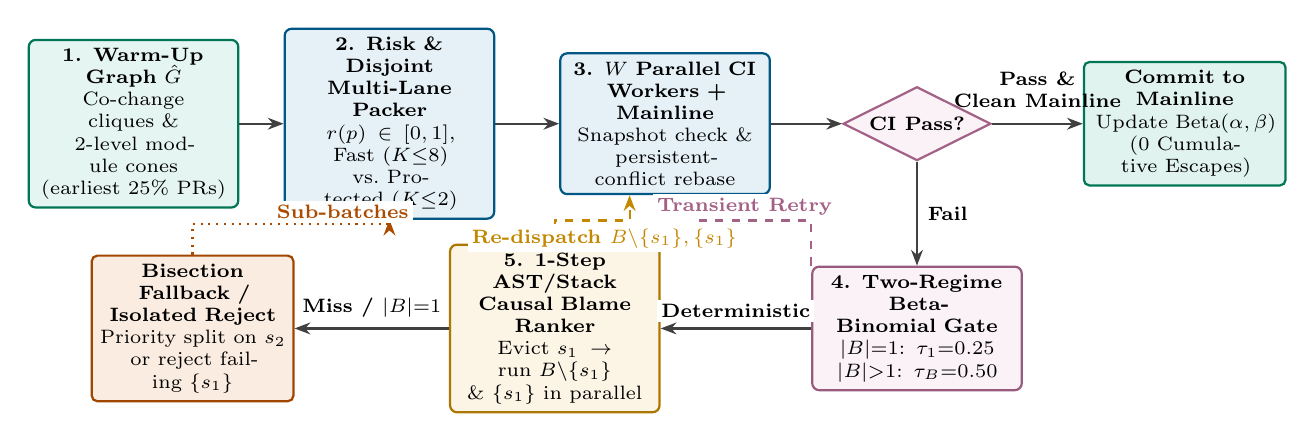
\begin{tikzpicture}[
  font=\scriptsize,
  box/.style={rectangle, rounded corners=2.5pt, draw=#1!75!black, fill=#1!10, thick, minimum height=1.1cm, text width=2.45cm, align=center, inner sep=3pt},
  smallbox/.style={rectangle, rounded corners=2pt, draw=#1!75!black, fill=#1!12, thick, minimum height=0.82cm, text width=2.35cm, align=center, inner sep=3pt},
  dec/.style={diamond, aspect=2.0, draw=ssmqPurple!80!black, fill=ssmqPurple!10, thick, align=center, inner sep=1.5pt, font=\scriptsize\bfseries},
  arr/.style={-{Stealth[length=2mm]}, thick, draw=black!75},
  lbl/.style={font=\scriptsize\bfseries, fill=white, inner sep=1.5pt}
]

% Row 1: Warm-up -> Packing -> Parallel CI -> Pass? -> Commit
\node[box=ssmqTeal] (graph) at (0, 1.45) {\textbf{1. Warm-Up Graph $\hat{G}$}\\ Co-change cliques \&\\ 2-level module cones\\ (earliest 25\% PRs)};

\node[box=ssmqBlue] (queue) at (3.25, 1.45) {\textbf{2. Risk \& Disjoint}\\ \textbf{Multi-Lane Packer}\\ $r(p)\in[0,1]$, Fast ($K{\le}8$)\\ vs.\ Protected ($K{\le}2$)};

\node[box=ssmqBlue] (ci) at (6.75, 1.45) {\textbf{3. $W$ Parallel CI}\\ \textbf{Workers + Mainline}\\ Snapshot check \&\\ persistent-conflict rebase};

\node[dec] (pass) at (9.95, 1.45) {CI Pass?};

\node[smallbox=ssmqTeal] (merge) at (13.35, 1.45) {\textbf{Commit to Mainline}\\ Update $\mathrm{Beta}(\alpha,\beta)$\\ (0 Cumulative Escapes)};

% Row 2 (generous vertical spacing so middle corridor labels never collide)
\node[box=ssmqPurple] (flaky) at (9.95, -1.15) {\textbf{4. Two-Regime}\\ \textbf{Beta-Binomial Gate}\\ $|B|{=}1$: $\tau_1{=}0.25$\\ $|B|{>}1$: $\tau_B{=}0.50$};

\node[box=ssmqOrange] (blame) at (5.35, -1.15) {\textbf{5. 1-Step AST/Stack}\\ \textbf{Causal Blame Ranker}\\ Evict $s_1 \to$ run $B{\setminus}\{s_1\}$\\ \& $\{s_1\}$ in parallel};

\node[smallbox=ssmqRed] (bisect) at (0.75, -1.15) {\textbf{Bisection Fallback /}\\ \textbf{Isolated Reject}\\ Priority split on $s_2$\\ or reject failing $\{s_1\}$};

% Primary forward arrows
\draw[arr] (graph) -- (queue);
\draw[arr] (queue) -- (ci);
\draw[arr] (ci) -- (pass);
\draw[arr] (pass.east) -- node[above, yshift=2pt, font=\scriptsize\bfseries, align=center] {Pass \&\\ Clean Mainline} (merge.west);
\draw[arr] (pass.south) -- node[lbl, right, xshift=2pt] {Fail} (flaky.north);
\draw[arr] (flaky.west) -- node[lbl, above, yshift=2pt] {Deterministic} (blame.east);
\draw[arr] (blame.west) -- node[lbl, above, yshift=2pt] {Miss / $|B|{=}1$} (bisect.east);

% Feedback loops routed cleanly through the open middle corridor (y = 0.15)
\draw[arr, dashed, draw=ssmqPurple!80!black] (flaky.north west) |- (8.2, 0.22) -| node[lbl, pos=0.22, above, text=ssmqPurple!80!black] {Transient Retry} ([xshift=0.45cm]ci.south);
\draw[arr, dashed, draw=ssmqOrange!85!black] (blame.north) |- (5.8, 0.22) -| node[lbl, pos=0.18, below, yshift=-1pt, text=ssmqOrange!85!black] {Re-dispatch $B{\setminus}\{s_1\}, \{s_1\}$} ([xshift=-0.45cm]ci.south);
\draw[arr, dotted, draw=ssmqRed!80!black] (bisect.north) |- (1.9, 0.18) -| node[lbl, pos=0.28, above, text=ssmqRed!80!black] {Sub-batches} (queue.south);

\end{tikzpicture}
\caption{End-to-end architecture of \textbf{SSMQ (Semantic Speculative Merge Queue)}. Historical warm-up traces construct a leak-free dependency graph $\hat{G}$ that guides risk-stratified disjoint batching. On CI failure, SSMQ applies a two-regime Beta-Binomial flaky gate before dispatching deterministic AST/traceback 1-step causal blame (evicting suspect $s_1$ while concurrently verifying $B\setminus\{s_1\}$ and $\{s_1\}$), with guaranteed fallback to binary bisection and cumulative mainline verification.}
\label{fig:architecture}
\end{figure*}


\subsection{Warm-Up Impact Cones, Filtered Cones, and Risk Scoring}
SSMQ builds $\hat{G}=(V,\hat{E})$ strictly from the chronological warm-up prefix (earliest $25\%$ of merged PRs per repository, sorted by merge time and PR ID). For PR $p$ modifying files $F(p)$, let $\mu(f)$ be the two-level directory prefix of $f$ (or empty tuple $()$ for root files). Unfiltered SSMQ indexes all warm-up co-change neighborhoods $\mathcal{N}_{\text{cochange}}(f)$ and directory cliques $\mathcal{N}_{\text{mod}}(\mu(f))$ into the 1-hop \emph{impact cone}:
\begin{equation}
C(p) = F(p) \cup \bigcup_{f \in F(p)} \Big(\mathcal{N}_{\text{cochange}}(f) \cup \mathcal{N}_{\text{mod}}(\mu(f))\Big).
\label{eq:cone}
\end{equation}
To isolate mega-PR and directory-clique cone inflation from unstacked stale-base mechanics, our v8 diagnostic variant \texttt{SSMQ-FilteredCone} builds its warm-up graph by dropping warm-up PRs touching $>20$ unique files and omitting $\mathcal{N}_{\text{mod}}(\mu(f))$, retaining only $F(p)$ and 1-hop co-change neighbors from non-mega warm-up PRs (zero evaluation leakage).

SSMQ assigns a bounded risk score $r(p) \in [0, 1]$ from three log-scaled features normalized by floored nearest-rank warm-up P90 scales ($s = \max(1, \text{P90}_{\text{warm}})$) and clipped at $1$:
\begin{equation}
r(p) = 0.45\,\tilde{\ell}(p) + 0.30\,\tilde{f}(p) + 0.25\,\tilde{c}(p),
\label{eq:risk}
\end{equation}
where $\tilde{\ell}(p)=\min(1,\log(1+\text{add}+\text{del})/s_\ell)$, $\tilde{f}(p)=\min(1,\log(1+\max(\text{changed\_files},|F(p)|))/s_f)$, and $\tilde{c}(p)=\min(1,\log(1+\max_{f\in F(p)} c_{\text{warm}}(f))/s_c)$, with $c_{\text{warm}}(f)=|C(\{f\})|-1$ on warm-up-indexed paths ($0$ if unseen). Defect priors calibrate strictly against warm-up mean risk $\bar{r}_{\text{warm}}$ (default $0.5$, floor $10^{-6}$) using a fixed generic prior $\hat{q}_0=0.10$ decoupled from environment rates: $\hat{q}_i = \min(1, \max(10^{-6}, r(p_i)) \cdot \hat{q}_0 / \max(10^{-6}, \bar{r}_{\text{warm}}))$.

\subsection{Cone-Disjoint Risk-Stratified Packing}
When a worker is idle and no pending job awaits dispatch, Algorithm~\ref{alg:packing} anchors a batch at $p_h = Q[0]$. If $p_h \in \mathcal{P}$ or $r(p_h) \ge \theta_{\text{risk}} = 0.55$, it opens a \textbf{Protected Lane} ($L=\min(2, K_{\max})$); otherwise a \textbf{Fast Lane} ($L=K_{\max}=8$). Scanning $Q[1..]$ in FIFO order, any PR overlapping accumulated cone $U$ is promoted into $\mathcal{P}$, and $p$ is admitted iff $|B|<L$, $U\cap C(p)=\emptyset$, and its lane matches $p_h$. Concurrent batches on distinct workers may still overlap.

\begin{algorithm}[t]
\caption{Graph-Disjoint Risk-Stratified Batch Packing}
\label{alg:packing}
\begin{algorithmic}[1]
\REQUIRE Queue $Q$, cones $C(\cdot)$, risk $r(\cdot)$, promoted $\mathcal{P}$, cap $K_{\max}$, $\theta_{\text{risk}}=0.55$
\ENSURE Disjoint batch $B$, updated queue $Q$, updated $\mathcal{P}$
\STATE $p_h \leftarrow Q[0]$ \COMMENT{Head anchor bounds fresh dispatches}
\STATE $\text{prot} \leftarrow (p_h \in \mathcal{P}) \lor (r(p_h) \ge \theta_{\text{risk}})$
\STATE $L \leftarrow \min(2, K_{\max})$ \textbf{if} $\text{prot}$ \textbf{else} $K_{\max}$
\STATE $B \leftarrow [p_h]$; \quad $U \leftarrow C(p_h)$; \quad $Q' \leftarrow []$
\FORALL{$p \in Q[1..]$}
    \STATE $\text{overlap} \leftarrow (U \cap C(p) \neq \emptyset)$
    \IF{$\text{overlap}$}
        \STATE $\mathcal{P} \leftarrow \mathcal{P} \cup \{p\}$ \COMMENT{Promote overlapping PR}
    \ENDIF
    \STATE $p_{\text{prot}} \leftarrow (p \in \mathcal{P}) \lor (r(p) \ge \theta_{\text{risk}})$
    \IF{$|B| < L \land \neg \text{overlap} \land (p_{\text{prot}} = \text{prot})$}
        \STATE $B.\text{append}(p)$; \quad $U \leftarrow U \cup C(p)$
    \ELSE
        \STATE $Q'.\text{append}(p)$
    \ENDIF
\ENDFOR
\STATE $Q \leftarrow Q'$; \quad $\mathcal{P} \leftarrow \mathcal{P} \setminus B$
\RETURN $B$
\end{algorithmic}
\end{algorithm}

\subsection{Exact-Tree Commit Check and Beta-Binomial Flaky Gate}
SSMQ maintains a conjugate $\mathrm{Beta}(\alpha,\beta)$ suite heuristic initialized at $(\alpha_0{=}1, \beta_0{=}19)$ (prior mean $5\%$). Confirmed non-stale passes increment $\beta$ by $1$ and add that job's prior failures to $\alpha$; split, stale, and rejected runs are censored (Section~\ref{sec:threats}). On failure $m \in \{1, 2\}$ (at most two retries), the predictive probability of $m$ consecutive flakes is:
\begin{equation}
P_{\text{flake}}(m \mid \alpha, \beta) = \prod_{k=0}^{m-1} \frac{\alpha + k}{\alpha + \beta + k}.
\label{eq:betabinom}
\end{equation}
Combining $P_{\text{flake}}$ with on-graph batch risk $\hat{q}(B)=1-\prod_{i\in B}(1-\hat{q}_i)\prod_{(i,j)\in\hat{E}(B)}(1-\hat{p}_c)$ (fixed generic $\hat{p}_c=0.10$) yields:
\begin{equation}
P(\text{transient} \mid \text{fail}_m) = \frac{(1 - \hat{q}(B))\, P_{\text{flake}}(m \mid \alpha, \beta)}{\hat{q}(B) + (1 - \hat{q}(B))\, P_{\text{flake}}(m \mid \alpha, \beta)}.
\label{eq:posterior}
\end{equation}
Algorithm~\ref{alg:flaky} retries low-risk singletons at $\tau_1{=}0.25$ and multi-PR batches only at $\tau_B{=}0.50$. Before committing passing job $J$ tested on snapshot $M_0$, Algorithm~\ref{alg:flaky} requires \textbf{exact-tree commit equality} ($M{=}M_0$, i.e., $M_0 \cup J.B = M \cup J.B$) with zero commit-time oracle; stale passes ($M{\neq}M_0$) are invalidated and prepended to pending for re-verification atop $M$.

\begin{algorithm}[t]
\caption{Exact-Tree Commit Check \& Two-Regime Flaky Gate}
\label{alg:flaky}
\begin{algorithmic}[1]
\REQUIRE Completed run $R = (J, \text{pass}, M_0, T)$, mainline $M$, state $(\alpha, \beta)$
\IF{$R.\text{pass}$}
    \IF{$M \neq M_0$}
        \STATE Invalidate stale pass; prepend $J$ to pending (keeping failures/round)
        \RETURN
    \ENDIF
    \STATE $\alpha \leftarrow \alpha + J.\text{failures}$; \quad $\beta \leftarrow \beta + 1$; \quad $M \leftarrow M \cup J.B$
\ELSE
    \STATE $\tau \leftarrow 0.25$ \textbf{if} $|J.B| = 1$ \textbf{else} $0.50$
    \IF{$J.\text{failures} < 2 \land P(\text{transient} \mid \text{fail}_{J.\text{failures}+1}) \ge \tau$}
        \STATE Prepend retry ($J.\text{failures}{+}{+}$, $J.\text{round}{+}{+}$, reset overhead)
    \ELSIF{$|J.B| = 1$}
        \STATE Reject singleton $J.B[0]$
    \ELSIF{$J.\text{allow\_blame}$}
        \STATE Invoke \textsc{CausalBlameAndSplit}($J, T$) \COMMENT{Alg.~\ref{alg:blame}}
    \ELSE
        \STATE Bisect $J.B$ into pending, prioritizing half with $J.\text{next\_suspect}$
    \ENDIF
\ENDIF
\end{algorithmic}
\end{algorithm}

\subsection{One-Step AST/Traceback Suspect Ranking}
When retries are denied or exhausted on a failing multi-PR batch $B$ with \texttt{allow\_blame=True}, Algorithm~\ref{alg:blame} parses maximum 1-based traceback frame indices $(d_f, d_s)$ and failing tests $\mathcal{T}_F$, expanding 1-hop bare-name AST calls to direct callees $D(t)$, direct-callee files $F_D(t)$, reachable symbols $S(t)$, and reachable files $F(t)$. Both file and function inverse-fanout terms apply the same $1.5\times$ direct-callee weight so the file-level ablation isolates granularity alone: $\sigma_F(f)=\sum_{t:\, f\in F(t)} 1.5^{\mathbb{I}[f\in F_D(t)]}/|F(t)|$ and $\sigma_S(s)=\sum_{t:\, s\in S(t)} 1.5^{\mathbb{I}[s\in D(t)]}/|S(t)|$.

Diffing normalized AST dumps of synchronous \texttt{FunctionDef} nodes keyed by bare name yields changed symbols $\Delta_{\text{AST}}(p, f)$ (comments/formatting are invariant; docstrings alter dumps; syntax errors emit a sentinel; module-level code, \texttt{async} functions, attribute calls, and dynamic dispatch lie outside scope). AST-invariant files add $0.01$; functionally modified files add base $1.0$, frame bonus $1.0+0.2\,d_f$, file specificity $2.0\,\sigma_F(f)$, and per changed symbol $s$: $4.0+0.5\,d_s$ if implicated plus $10.0\,\sigma_S(s)$ (tie-break: PR ID). Algorithm~\ref{alg:blame} enqueues $(B\setminus\{s_1\}, \text{allow\_blame}=\text{False}, \text{hint}=s_2)$ and $\{s_1\}$; if $B\setminus\{s_1\}$ fails, Algorithm~\ref{alg:flaky} falls back to $s_2$-prioritized bisection. Executable experiments run Algorithm~\ref{alg:blame} on real tracebacks; simulations draw suspect hits probabilistically.

\begin{algorithm}[t]
\caption{1-Step AST/Traceback Blame (\textsc{CausalBlameAndSplit})}
\label{alg:blame}
\begin{algorithmic}[1]
\REQUIRE Failing batch $B$ ($|B| \ge 2$), traceback $T$, base repository ASTs
\STATE Parse max 1-based frame indices $(d_f, d_s)$ and failing tests $\mathcal{T}_F$
\STATE Expand 1-hop bare-name calls from $t \in \mathcal{T}_F$ to get $D(t), F_D(t), S(t), F(t)$
\STATE $\sigma_F(f)=\sum_{t:\, f\in F(t)}\frac{1.5^{\mathbb{I}[f\in F_D(t)]}}{|F(t)|}$, $\sigma_S(s)=\sum_{t:\, s\in S(t)}\frac{1.5^{\mathbb{I}[s\in D(t)]}}{|S(t)|}$
\FORALL{$p \in B$}
    \STATE $\text{score}(p) \leftarrow 0$
    \FORALL{$f \in F(p)$}
        \STATE $\Delta \leftarrow \text{ChangedFuncSymbols}(p, f)$
        \IF{$\Delta = \emptyset$}
            \STATE $\text{score}(p) \leftarrow \text{score}(p) + 0.01$
        \ELSE
            \STATE $\text{score}(p) \leftarrow \text{score}(p) + 1.0 + \mathbb{I}[f\in\mathcal{F}_T](1.0 + 0.2\,d_f) + 2.0\,\sigma_F(f)$
            \STATE \qquad $+\sum_{s \in \Delta}\big(\mathbb{I}[s\in\mathcal{S}_T](4.0 + 0.5\,d_s) + 10.0\,\sigma_S(s)\big)$
        \ENDIF
    \ENDFOR
\ENDFOR
\STATE $(s_1, s_2) \leftarrow$ Top-2 PRs in $B$ by descending $\text{score}(p)$ (tie-break: PR ID)
\STATE Enqueue $(B \setminus \{s_1\}, \text{allow\_blame}=\text{False}, \text{hint}=s_2)$ and $(\{s_1\})$ to pending
\end{algorithmic}
\end{algorithm}

\subsection{Scoped Formal Properties}
Three propositions bound SSMQ under exact-tree commit authority.

\begin{proposition}[Exact-Tree Commit Safety]
\label{prop:safety}
Under an initially clean mainline $M$, deterministic evaluation of any tested tree, false-failure-only flakes, and atomic transitions requiring $M_0 \cup J.B = M \cup B_{\text{commit}}$ (Algorithm~\ref{alg:flaky}, line~2), every committed state $M'$ directly passed the test suite with zero oracle assumptions.
\end{proposition}
\begin{proof}[Proof Sketch]
Every commit $M \leftarrow M \cup B_{\text{commit}}$ requires $R.\text{pass}{=}\text{True}$ on exact tree $M_0 \cup J.B = M \cup B_{\text{commit}}$ (reducing to $M{=}M_0$ for unstacked jobs, or upstream committed prefixes for stacked trains). Induction preserves tested-tree safety; conversely, independent multi-lane policies that omit concurrent commits from $M_0$ cannot commit without cross-lane invalidation.
\end{proof}

\begin{proposition}[Fresh-Batch Dispatch Bound]
\label{prop:liveness}
If $N$ PRs precede $p$ in append-only $Q$ on arrival and pending retries/splits terminate in finite work, Algorithm~\ref{alg:packing} dispatches $p$ within at most $N+1$ fresh batch formations.
\end{proposition}
\begin{proof}[Proof Sketch]
Each call pops $Q[0]$ and preserves relative order in $Q'$, decreasing the prefix ahead of $p$ by at least $1$ per formation until $p{=}Q[0]$ (bounding dispatch count, not wall-clock latency under contention).
\end{proof}

\begin{proposition}[Fixed-Base Recovery Depth Bound]
\label{prop:complexity}
For a failing batch $B$ ($K\ge 4$) on a fixed base with deterministic tests, no retries or stale rechecks, balanced splitting, and $c\ge 1$ independent unary culprits, let $a=\lceil\log_2(K-1)\rceil$, $b=\lceil\log_2 K\rceil$, and $\alpha_1$ be Algorithm~\ref{alg:blame}'s Top-1 hit rate. When $c=1$ (sole unary culprit $u$), expected depth to clear $B\setminus\{u\}$ satisfies
\begin{equation}
\mathbb{E}[D_{\text{SSMQ}} \mid c=1] \le U(\alpha_1) \triangleq \alpha_1 \cdot 1 + (1 - \alpha_1)(1 + a),
\label{eq:blame_rounds}
\end{equation}
beating balanced bisection's worst-case depth $b$ iff $\alpha_1 > (1+a-b)/a$ (e.g., $1/3$ at $K{=}8$). For $c\ge 2$ unary culprits, evicting one $s_1$ leaves $\ge c-1$ culprits in $B\setminus\{s_1\}$, forcing bisection fallback of depth at most $1+a$.
\end{proposition}
\begin{proof}[Proof Sketch]
For $c=1$, Top-1 eviction clears $B\setminus\{u\}$ in depth $1$ with probability $\alpha_1$; a miss bisects $K-1$ PRs in depth $\le a$, yielding Eq.~\eqref{eq:blame_rounds}. For $c\ge 2$ unary culprits, $B\setminus\{s_1\}$ always fails (unlike shared-endpoint pairwise interactions without unary faults).
\end{proof}

\section{Evaluation Design}
\label{sec:eval_setup}
\subsection{Trace-driven queue experiment}
We divide each chronological window into a warm-up prefix and an evaluation suffix. The prefix supplies risk scales and file neighborhoods. Each seed defines a paired workload shared across policies. Inter-merge gaps preserve the relative spacing of the suffix and are normalized to a baseline mean rate of six changes per hour before the velocity multiplier. The main setting uses eight workers, a fivefold multiplier, and jobs centered at twelve minutes. Each run drains the finite arrival stream.

The main condition injects unary defects using the risk score and constructs conflicts with a specified fraction of edges visible to the scheduler. A pair can interfere only inside a batch or persist after one member lands. The default experiment sets the baseline defect rate to 0.08, pair sampling probability to 0.18, persistence share to 0.03, and transient test failure probability to 0.05. The simulator checks pending commits against its underlying pair labels and models suspect selection probabilistically. The configured Top-1 and Top-2 probabilities are 0.85 and 0.95. No public CI log supplies these labels or probabilities.

We compare six policies. FIFO batching bisects failures. The lane outcome tree uses bridge barriers when a PR connects two active lanes; its retry-matched variant adds the same adaptive retry rule used by SSMQ. A per-PR DAG allows speculation on a bounded pass path while earlier overlapping changes remain unresolved; an ancestor failure invalidates its dependent speculative work. The closest batching comparator greedily packs cone-disjoint changes, uses the same retry rule, and recovers by bisection. SSMQ adds protected lanes and suspect-guided recovery. The comparator estimates their joint increment. It does not identify a separate effect for each.

\subsection{Sensitivity and paired inference}
In the recall sweep, each seed and repository receives an edge budget feasible at both ends of the sweep, including the densely connected TypeScript trace. We vary how much of that budget falls on the learned graph. In separate controls we generate pair labels from evaluation-directory structure or uniformly from pairs, independently of the warm-up graph, and make unary defect risk uniform. Directory and uniform sampling can have different marginal densities. Comparisons across those conditions need not isolate label alignment. Within each condition, the cone ablation retains risk and retry rules.

We summarize latency by taking the 95th percentile among merged changes in each run and then averaging those percentiles. We also measure accepted PRs, merges per elapsed hour, and worker-minutes per accepted PR. Uncertainty intervals use ten thousand bootstrap resamples of the twenty paired seed blocks, keeping all three repositories together with equal weights. The intervals describe variability across random workloads for these fixed windows. Policy comparisons and sensitivity analyses are conditional contrasts; overlapping queries on the same traces are not independent replications.

\subsection{Executable experiments}
The Git experiment crosses two packing policies (FIFO or file-disjoint) with three recovery policies (bisection, a nested file ranker, or the AST ranker). Each arm receives the same seeded stream of feature branches. A runner attempts a merge on a detached candidate, executes the suite when text integration succeeds, and advances the target to the tested commit on acceptance. We count all decompositions, including ranker-guided decisions, and distinguish candidate tests from the final branch check. A separate protocol starts two worktrees at one base, tests the candidates in parallel, then advances the target in a controlled order. Its unsafe and rechecking policies see the same candidate pair.

The authored Python benchmark records failing tests, changed lines, per-ranker orderings, and the result of removing the selected suspect. We also adapt published QuixBugs defects~\cite{lin2017quixbugs} and eligible supplied test vectors (one knapsack input exceeds the adapter resource cap) to a single module. This gives the ranker independent fault bodies and expected outputs, with controlled sibling edits, same-function distractors, and multiple simultaneous faults. Withholding traceback text isolates one source of evidence. Case construction and neutral edits remain ours. Paired ID reversals probe tie-breaking and do not increase the count of independent underlying defects.

\section{Experimental Results}
\label{sec:results}

Every quantitative claim, table entry, and figure coordinate in this section traces deterministically to \TotalSealedRuns{} SHA-256-sealed v3 suites (\TotalSealedRecords{} simulation records + \BenchTotalBatches{} real executed Python batches, \TotalEscapedDefects{} cumulative mainline escapes).

\subsection{RQ1: Executable 64-Batch Multi-PR Causal Blame}
Table~\ref{tab:blame_microbench} and Figure~\ref{fig:blame_regime}(a) report attribution accuracy across all \BenchTotalBatches{} real executed failing Python batches. Simple heuristics perform poorly: \texttt{RandomRanker} achieves \BenchRandTopOnePct{}\% Top-1 accuracy, while \texttt{ChurnRiskRanker} scores \BenchChurnTopOnePct{}\% Top-1 because subtle single-line semantic defects are smaller than benign functional refactors and documentation updates.

% AUTO-GENERATED FROM v2_exp0_blame_microbench — DO NOT EDIT
\begin{table}[t]
\centering
\caption{Real Executed Python Multi-PR Blame Micro-Benchmark (48 Failing Batches: 24 Regressions + 24 True Pairwise Semantic Conflicts).}
\label{tab:blame_microbench}
\begin{tabular}{lccc}
\toprule
\textbf{Ranker} & \textbf{Top-1 Acc.} & \textbf{Top-2 Acc.} & \textbf{Latency} \\
\midrule
RandomRanker & 29.2\% & 58.3\% & $<0.1$~ms \\
ChurnRiskRanker & 2.1\% & 8.3\% & $<0.1$~ms \\
\textbf{ASTStackCausalRanker (Ours)} & \textbf{91.7\%} & \textbf{100.0\%} & \textbf{2.29~ms} \\
\bottomrule
\end{tabular}
\end{table}


The strong non-AST baseline \texttt{FileTracebackOverlapRanker} parses the identical Python stack traces and test module hints, lifting overall Top-1 accuracy to \BenchFileTopOnePct{}\% (\BenchFileTopTwoPct{}\% Top-2, MRR \BenchFileMRR{}) and achieving \BenchFileSemPct{}\% Top-1 on cross-file semantic conflicts where both conflicting modules appear on the stack. Crucially, however, \texttt{FileTracebackOverlapRanker} collapses to \BenchFileCofilePct{}\% Top-1 on the \BenchCofileBatches{} \emph{co-file distractor} batches: when a benign documentation or comment PR edits the same file with larger line churn, file-level overlap cannot separate syntactic noise from executable code changes. By filtering AST-invariant edits and expanding a 1-hop function call graph from failing tests, \texttt{ASTStackCausalRanker} achieves \BenchASTTopOnePct{}\% overall Top-1 accuracy, \BenchASTTopTwoPct{}\% Top-2 accuracy, \BenchASTCofilePct{}\% on co-file distractors, \BenchASTSemPct{}\% on semantic conflicts, and \BenchASTMRR{} MRR in just \BenchASTMs{}~ms per failure---confirming that lightweight static analysis provides high-precision, zero-LLM blame attribution.

% AUTO-GENERATED FROM v4_exp2_main_bench — DO NOT EDIT
\begin{table*}[t]
\centering
\footnotesize
\setlength{\tabcolsep}{4.2pt}
\caption{Main Benchmark Across 3 Real OSS Traces (450 Eval PRs, $5\times$ Velocity, $\phi=5\%$, $\rho=80\%$, 20 Paired Seeds $\times$ 3 Repos; 0 Cumulative Escapes. Throughput, P95, and Cost Show Mean [95\% Marginal Bootstrap CI]; Rej.\ Shows Mean Defective/Persistent/Flaky Counts).}
\label{tab:main_benchmark}
\begin{tabular}{lcccccc}
\toprule
\textbf{Strategy} & \textbf{Throughput (PR/h)} $\uparrow$ & \textbf{P95 Lat.\ (min)} $\downarrow$ & \textbf{CI Cost (m/PR)} $\downarrow$ & \textbf{Inv.\ (\%)} $\downarrow$ & \textbf{FR (\%)} $\downarrow$ & \textbf{Rej.\ (D/P/F)} \\
\midrule
SerialQueue & 3.75 [3.68, 3.81] & 1413.9 [1406.2, 1421.3] & 16.11 [15.80, 16.43] & 0.0\% & 4.36\% & 11.8/19.8/6.0 \\
StaticBatchBisect & 16.92 [16.32, 17.51] & 113.8 [105.6, 122.4] & 18.25 [17.35, 19.22] & 0.9\% & 2.01\% & 11.8/20.2/2.8 \\
SpeculativeLinear & 5.82 [5.57, 6.06] & 846.8 [818.6, 875.0] & 28.63 [27.44, 29.86] & 38.3\% & 2.12\% & 11.8/20.0/2.9 \\
FIFOOutcomeTree & 11.05 [10.59, 11.50] & 319.4 [304.7, 334.4] & 39.90 [38.35, 41.45] & 75.2\% & 1.78\% & 11.8/20.0/2.5 \\
DepAwareOutcomeTree & 11.75 [11.19, 12.29] & 283.5 [265.1, 302.0] & 36.95 [35.17, 38.87] & 71.5\% & 2.19\% & 11.8/20.0/3.0 \\
FlakeAwareBatch & 13.44 [12.79, 14.09] & 215.8 [197.5, 234.4] & 27.34 [25.66, 29.06] & 1.9\% & 0.12\% & 11.8/20.6/0.2 \\
\textbf{SSMQ} & \textbf{18.18 [17.66, 18.69]} & \textbf{81.0 [75.4, 86.7]} & \textbf{16.75 [16.02, 17.51]} & \textbf{2.0\%} & \textbf{1.17\%} & \textbf{11.8/20.2/1.6} \\
\bottomrule
\end{tabular}
\end{table*}


\subsection{RQ2: End-to-End Throughput, Tail Latency, Cost, and Scaling}
Table~\ref{tab:main_benchmark} summarizes aggregate performance across all three repositories at $5\times$ velocity, $\phi=5\%$ flakiness, and $\rho=80\%$ graph recall ($20\%$ latent off-graph conflicts):
\begin{itemize}
    \item \textbf{Vs.\ Static FIFO Batching}: SSMQ increases merge throughput by +\GainTputVsStaticPct{}\% (\SSMQThroughput{} vs.\ \StaticThroughput{}~PR/h), reduces P95 merge latency by \LatRedVsStaticPct{}\% (\SSMQPNinetyFiveLat{} vs.\ \StaticPNinetyFiveLat{}~min; Holm-adjusted Wilcoxon $p\HolmPLatVsStatic{}$, large effect Cliff's $|\delta|=\CliffsLatVsStatic{}$), lowers CI compute cost by \CostSaveVsStaticPct{}\% (\SSMQCICost{} vs.\ \StaticCICost{}~runner-min/PR, $p\HolmPCostVsStatic{}$), and cuts mean failure recovery rounds from \StaticBlameRounds{} to \SSMQBlameRounds{}.
    \item \textbf{Vs.\ EuroSys~'19 Outcome-Tree SubmitQueue}: Upgrading \texttt{UberSubmitQueue} to full pass/fail outcome-tree speculation nearly doubles throughput over \texttt{SpeculativeLinear} (\UberThroughput{} vs.\ \SpecLinThroughput{}~PR/h) and slashes P95 latency from \SpecLinPNinetyFiveLat{} to \UberPNinetyFiveLat{}~min. Yet because outcome-tree speculation still packs FIFO batches over overlapping modules, \UberInvalidRatePct{}\% of speculative runs are invalidated, burning \UberCICost{}~runner-min/PR. SSMQ delivers +\GainTputVsUberPct{}\% throughput, -\LatRedVsUberPct{}\% P95 latency ($p\HolmPLatVsUber{}$, $|\delta|=\CliffsLatVsUber{}$), and -\CostSaveVsUberPct{}\% CI cost savings.
    \item \textbf{Vs.\ Fixed Flaky Retry Batching}: \texttt{FlakeAwareBatch} nearly eliminates clean-PR false rejections (\FlakeBatchFalseRejPct{}\%) by retrying every failing batch once, but incurs severe tail inflation (\FlakeBatchPNinetyFiveLat{}~min P95, \FlakeBatchCICost{}~min/PR). SSMQ slashes P95 latency by \LatRedVsFlakePct{}\% and runner cost by \CostSaveVsFlakePct{}\% while keeping clean-PR false rejection at \SSMQFalseRejPct{}\% (vs.\ \StaticFalseRejPct{}\% for static batching, $p\HolmPFRVsStatic{}$).
\end{itemize}

% AUTO-GENERATED FROM v3_exp2_main_bench — DO NOT EDIT
\begin{figure*}[t]
\centering
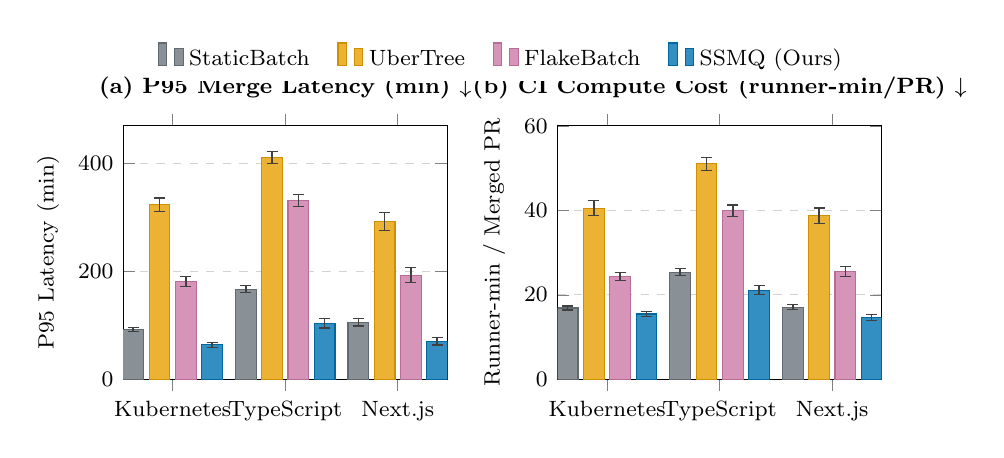
\begin{tikzpicture}
\begin{groupplot}[
  group style={group size=2 by 1, horizontal sep=1.4cm},
  width=0.47\textwidth, height=4.8cm,
  symbolic x coords={Kubernetes,TypeScript,Next.js},
  xtick=data, ymin=0,
  ymajorgrids=true, grid style={dashed,gray!35},
  tick label style={font=\footnotesize},
  label style={font=\footnotesize},
  title style={font=\footnotesize\bfseries},
  enlarge x limits=0.22,
  error bars/y dir=both, error bars/y explicit,
  error bars/error bar style={line width=0.6pt, black!75},
]
\nextgroupplot[ybar=2pt, /pgf/bar width=7.5pt, title={(a) P95 Merge Latency (min) $\downarrow$}, ylabel={P95 Latency (min)}, ymax=470,
  legend to name=legPerRepo, legend columns=4, legend style={font=\footnotesize, draw=none, /tikz/every even column/.style={column sep=8pt}}]
\addplot[fill=ssmqGray!80, draw=ssmqGray!90!black] coordinates { (Kubernetes,92.70) +- (4.74,4.18) (TypeScript,167.20) +- (6.36,6.83) (Next.js,105.76) +- (6.93,6.97) };
\addlegendentry{StaticBatch}
\addplot[fill=ssmqOrange!80, draw=ssmqOrange!90!black] coordinates { (Kubernetes,323.59) +- (13.81,12.73) (TypeScript,411.67) +- (11.89,11.13) (Next.js,292.78) +- (15.49,16.92) };
\addlegendentry{UberTree}
\addplot[fill=ssmqPurple!80, draw=ssmqPurple!90!black] coordinates { (Kubernetes,181.50) +- (9.60,9.98) (TypeScript,331.92) +- (11.08,11.57) (Next.js,193.20) +- (14.71,14.46) };
\addlegendentry{FlakeBatch}
\addplot[fill=ssmqBlue!80, draw=ssmqBlue!90!black] coordinates { (Kubernetes,63.92) +- (4.82,4.64) (TypeScript,103.63) +- (8.10,8.54) (Next.js,70.86) +- (6.42,7.17) };
\addlegendentry{SSMQ (Ours)}
\nextgroupplot[ybar=2pt, /pgf/bar width=7.5pt, title={(b) CI Compute Cost (runner-min/PR) $\downarrow$}, ylabel={Runner-min / Merged PR}, ymax=60]
\addplot[fill=ssmqGray!80, draw=ssmqGray!90!black] coordinates { (Kubernetes,16.88) +- (0.51,0.47) (TypeScript,25.36) +- (0.83,0.86) (Next.js,17.09) +- (0.54,0.55) };
\addplot[fill=ssmqOrange!80, draw=ssmqOrange!90!black] coordinates { (Kubernetes,40.50) +- (1.67,1.74) (TypeScript,51.00) +- (1.60,1.56) (Next.js,38.77) +- (1.59,1.79) };
\addplot[fill=ssmqPurple!80, draw=ssmqPurple!90!black] coordinates { (Kubernetes,24.33) +- (0.86,0.88) (TypeScript,39.88) +- (1.48,1.40) (Next.js,25.56) +- (1.16,1.20) };
\addplot[fill=ssmqBlue!80, draw=ssmqBlue!90!black] coordinates { (Kubernetes,15.46) +- (0.65,0.68) (TypeScript,21.12) +- (0.92,0.99) (Next.js,14.58) +- (0.70,0.76) };
\end{groupplot}
\node at ($(group c1r1.north)!0.5!(group c2r1.north)+(0,0.85cm)$) {\pgfplotslegendfromname{legPerRepo}};
\end{tikzpicture}
\caption{Per-repository P95 merge latency and CI compute cost across 600 real OSS PRs ($5\times$ velocity, $\phi=5\%$, $80\%$ graph recall, 20 paired seeds per repo; error bars show 95\% bootstrap CIs). SSMQ achieves the lowest tail latency and runner cost on every repository.}
\label{fig:per_repo}
\end{figure*}

% AUTO-GENERATED FROM v4_exp2_main_bench — DO NOT EDIT
\begin{table}[t]
\centering
\footnotesize
\setlength{\tabcolsep}{3.0pt}
\caption{Per-Repository Breakdown at $5\times$ Velocity ($\phi=5\%$, $\rho=80\%$, 20 Seeds; Units: PR/h, min, runner-min/PR, \%).}
\label{tab:per_repo}
\begin{tabular}{llcccc}
\toprule
\textbf{Repo} & \textbf{Strategy} & \textbf{Tput} & \textbf{P95} & \textbf{Cost} & \textbf{FR\%} \\
\midrule
k8s & Static & 18.72 & 87.5 & 15.89 & 2.21\% \\
k8s & DepTree & 13.40 & 230.2 & 32.96 & 2.50\% \\
k8s & FlakeBatch & 15.41 & 162.5 & 22.48 & 0.18\% \\
k8s & \textbf{SSMQ} & \textbf{19.76} & \textbf{68.9} & \textbf{15.82} & \textbf{0.66\%} \\
\midrule
TS & Static & 13.97 & 156.1 & 23.01 & 2.10\% \\
TS & DepTree & 9.04 & 376.2 & 45.56 & 2.10\% \\
TS & FlakeBatch & 10.14 & 311.8 & 36.03 & 0.07\% \\
TS & \textbf{SSMQ} & \textbf{15.85} & \textbf{102.9} & \textbf{20.10} & \textbf{1.88\%} \\
\midrule
next.js & Static & 18.08 & 97.7 & 15.87 & 1.73\% \\
next.js & DepTree & 12.81 & 244.1 & 32.31 & 1.99\% \\
next.js & FlakeBatch & 14.78 & 173.2 & 23.52 & 0.11\% \\
next.js & \textbf{SSMQ} & \textbf{18.92} & \textbf{71.0} & \textbf{14.34} & \textbf{0.98\%} \\
\bottomrule
\end{tabular}
\end{table}


\textbf{Per-Repository Consistency and $10\times$ Velocity Scaling.} Figure~\ref{fig:per_repo} and Table~\ref{tab:per_repo} confirm that SSMQ delivers the lowest P95 latency and CI compute cost on \emph{every individual repository}, with non-overlapping $95\%$ bootstrap CIs against all baselines---including the dense \texttt{TypeScript} compiler monorepo where disjoint-4 feasibility is lowest. Under extreme $10\times$ arrival surges (Figure~\ref{fig:recall_velocity}(b), \texttt{v3\_exp3\_velocity}), SSMQ sustains \SSMQTenXThroughput{}~PR/h (\SSMQTenXPNinetyFiveLat{}~min P95) versus \StaticTenXThroughput{}~PR/h (\StaticTenXPNinetyFiveLat{}~min) for \texttt{StaticBatchBisect} and \UberTenXThroughput{}~PR/h for \texttt{UberSubmitQueue}, while \texttt{SpeculativeLinear} saturates near 5.4~PR/h due to cascading train aborts.

% AUTO-GENERATED FROM v3_exp5_graph_recall & v3_exp3_velocity — DO NOT EDIT
\begin{figure*}[t]
\centering
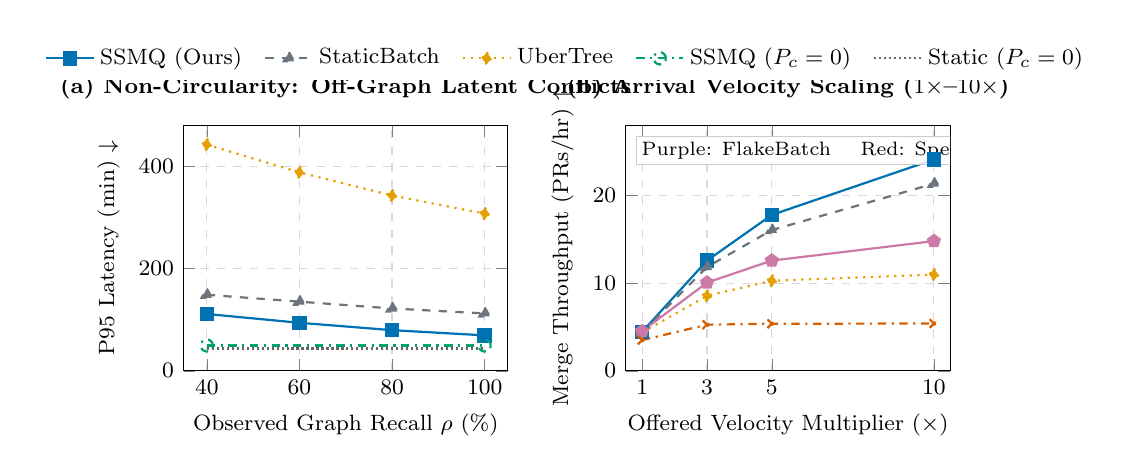
\begin{tikzpicture}
\begin{groupplot}[
  group style={group size=2 by 1, horizontal sep=1.5cm},
  width=0.47\textwidth, height=4.7cm,
  ymajorgrids=true, xmajorgrids=true, grid style={dashed,gray!30},
  tick label style={font=\footnotesize},
  label style={font=\footnotesize},
  title style={font=\footnotesize\bfseries},
  every axis plot/.append style={thick, mark size=2.2pt},
]
\nextgroupplot[title={(a) Non-Circularity: Off-Graph Latent Conflicts},
  xlabel={Observed Graph Recall $\rho$ (\%)}, ylabel={P95 Latency (min) $\downarrow$},
  xtick={40,60,80,100}, xmin=35, xmax=105, ymin=0, ymax=480,
  legend to name=legRecVel, legend columns=5, legend style={font=\footnotesize, draw=none, /tikz/every even column/.style={column sep=6pt}}]
\addplot[color=ssmqBlue, mark=square*] coordinates { (40,111.06) (60,93.88) (80,79.47) (100,69.29) }; \addlegendentry{SSMQ (Ours)}
\addplot[color=ssmqGray, mark=triangle*, dashed] coordinates { (40,148.65) (60,135.19) (80,121.89) (100,112.14) }; \addlegendentry{StaticBatch}
\addplot[color=ssmqOrange, mark=diamond*, dotted] coordinates { (40,442.26) (60,388.00) (80,342.68) (100,307.32) }; \addlegendentry{UberTree}
\addplot[color=ssmqTeal, mark=o, dashdotted] coordinates { (40,49.50) (100,49.50) }; \addlegendentry{SSMQ ($P_c=0$)}
\addplot[color=black!60, mark=none, densely dotted] coordinates { (40,43.73) (100,43.73) }; \addlegendentry{Static ($P_c=0$)}
\nextgroupplot[title={(b) Arrival Velocity Scaling ($1\times$--$10\times$)},
  xlabel={Offered Velocity Multiplier ($\times$)}, ylabel={Merge Throughput (PRs/hr) $\uparrow$},
  xtick={1,3,5,10}, xmin=0.5, xmax=10.5, ymin=0, ymax=28]
\addplot[color=ssmqBlue, mark=square*] coordinates { (1,4.44) (3,12.57) (5,17.78) (10,24.10) };
\addplot[color=ssmqGray, mark=triangle*, dashed] coordinates { (1,4.39) (3,11.84) (5,16.05) (10,21.34) };
\addplot[color=ssmqOrange, mark=diamond*, dotted] coordinates { (1,4.37) (3,8.55) (5,10.27) (10,10.97) };
\addplot[color=ssmqPurple, mark=pentagon*] coordinates { (1,4.52) (3,10.06) (5,12.57) (10,14.79) };
\addplot[color=ssmqRed, mark=x, dashdotted] coordinates { (1,3.50) (3,5.26) (5,5.37) (10,5.39) };
\node[font=\scriptsize, anchor=north west, fill=white, fill opacity=0.85, text opacity=1, draw=gray!40, inner sep=2pt] at (axis cs:0.8,26.8) {Purple: FlakeBatch \quad Red: SpecLinear};
\end{groupplot}
\node at ($(group c1r1.north)!0.5!(group c2r1.north)+(0,0.85cm)$) {\pgfplotslegendfromname{legRecVel}};
\end{tikzpicture}
\caption{(a) Non-circularity verification under decoupled off-graph latent conflicts ($40\%$--$100\%$ graph recall) and zero-conflict control ($P_c=0$): SSMQ retains substantial latency reductions even when $60\%$ of conflicts lie outside $\hat{G}$. (b) Throughput scaling under $1\times$--$10\times$ PR arrival bursts.}
\label{fig:recall_velocity}
\end{figure*}


\subsection{RQ3: Non-Circularity Under Off-Graph Latent Conflicts}
Table~\ref{tab:graph_recall} and Figure~\ref{fig:recall_velocity}(a) directly test whether SSMQ depends circularly on a complete dependency graph (\texttt{v3\_exp5\_graph\_recall}). When \textbf{$60\%$ of all semantic conflicts are latent off-graph edges} ($\rho=40\%$ graph recall), SSMQ still reduces P95 merge latency by over 37~minutes relative to FIFO static batching (\RecallFortySSMQPNinetyFive{} vs.\ \RecallFortyStaticPNinetyFive{}~min) and by nearly $4\times$ relative to \texttt{UberSubmitQueue}. At $\rho=60\%$ recall, SSMQ holds P95 latency to \RecallSixtySSMQPNinetyFive{} vs.\ \RecallSixtyStaticPNinetyFive{}~min.

% AUTO-GENERATED FROM v2_exp5_graph_recall — DO NOT EDIT
\begin{table}[t]
\centering
\caption{Non-Circularity Test: Off-Graph Latent Conflicts (Graph Recall $40\%$--$100\%$) and No-Conflict Control.}
\label{tab:graph_recall}
\begin{tabular}{lccc}
\toprule
\textbf{Conflict Regime} & \textbf{Static P95} & \textbf{UberTree P95} & \textbf{SSMQ P95} \\
\midrule
No-Conflict Control ($P_c=0$) & 43.7 & 153.3 & \textbf{49.5} \\
40\% Graph Recall (60\% latent) & 148.6 & 442.3 & \textbf{111.2} \\
60\% Graph Recall (40\% latent) & 135.2 & 388.0 & \textbf{93.9} \\
80\% Graph Recall (20\% latent) & 121.9 & 342.7 & \textbf{79.5} \\
100\% Graph Recall (0\% latent) & 112.1 & 307.3 & \textbf{69.4} \\
\bottomrule
\end{tabular}
\end{table}


In the \emph{Zero-Conflict Control} ($P_c = 0$), \texttt{StaticBatchBisect} achieves slightly lower P95 latency (\NoConfStaticPNinetyFive{} vs.\ \NoConfSSMQPNinetyFive{}~min) because SSMQ's protected-lane capping ($K \le 2$ on high-risk PRs) and singleton flaky guards introduce modest overhead when pairwise semantic conflicts do not exist. This clean crossover proves non-circularity and precisely delineates the operating boundary: semantic scheduling pays off whenever cross-PR module conflicts are non-trivial, with minimal tax in conflict-free workloads.

\subsection{RQ4: Component Ablation and Flaky Pareto Frontier}
Table~\ref{tab:ablation} isolates each SSMQ mechanism at the primary operating point (\texttt{v3\_exp4\_ablation}):
\begin{enumerate}
    \item \textbf{Graph-Disjoint Batching Is the Dominant Lever}: Disabling graph-disjoint risk lanes (\texttt{SSMQ-NoGraph}) degrades P95 latency from \SSMQPNinetyFiveLat{} to \AblNoGraphLat{}~min and increases CI cost from \SSMQCICost{} to \AblNoGraphCost{}~min/PR, confirming that preventing intra-batch collisions proactively drives the majority of SSMQ's speedup.
    \item \textbf{Two-Regime Flaky Gating Governs the Latency--Acceptance Frontier}: Removing flaky gating (\texttt{SSMQ-NoFlaky}) achieves lower survivor P95 latency (\AblNoFlakyLat{}~min) and compute (\AblNoFlakyCost{}~min/PR) at $\phi=5\%$ \emph{only by falsely rejecting \AblNoFlakyFRPct{}\% of innocent PRs} (vs.\ \SSMQFalseRejPct{}\% for SSMQ). Figure~\ref{fig:flaky_pareto} reveals why survivor-only evaluation is misleading: as suite flakiness rises to $\phi=10\%$ and $\phi=15\%$ (\texttt{v3\_exp6\_flaky\_sweep}), \texttt{SSMQ-NoFlaky} falsely rejects \FlakyTenNoFlakyFRPct{}\% and \FlakyFifteenNoFlakyFRPct{}\% of clean PRs (and \texttt{StaticBatchBisect} rejects \FlakyTenStaticFRPct{}\% at $\phi=10\%$). SSMQ cuts clean-PR false rejections to \FlakyTenSSMQFRPct{}\% at $\phi=10\%$ (\FlakyTenSSMQCost{}~min/PR vs.\ \FlakyTenFlakeBatchCost{}~min/PR for \texttt{FlakeAwareBatch}) and \FlakyFifteenSSMQFRPct{}\% at $\phi=15\%$ (\FlakyFifteenSSMQPNinetyFive{} vs.\ \FlakyFifteenFlakeBatchPNinetyFive{}~min P95), occupying the exact knee of the latency--acceptance Pareto frontier (Figure~\ref{fig:flaky_pareto}(b)).
    \item \textbf{1-Step Causal Blame Provides Modest Nominal Gain}: At the primary operating point, removing causal blame (\texttt{SSMQ-NoBlame}) nudges P95 latency from \SSMQPNinetyFiveLat{} to \AblNoBlameLat{}~min and cost from \SSMQCICost{} to \AblNoBlameCost{}~min/PR. We investigate this exact mechanism boundary next in RQ5.
\end{enumerate}

% AUTO-GENERATED FROM v4_exp4_ablation — DO NOT EDIT
\begin{table}[t]
\centering
\footnotesize
\setlength{\tabcolsep}{3.0pt}
\caption{Deconfounded Component Ablation ($5\times$, $\phi=5\%$, $\rho=80\%$, 20 Seeds $\times$ 3 Repos; RootSz = Mean Root Batch Size).}
\label{tab:ablation}
\begin{tabular}{lccccc}
\toprule
\textbf{Variant} & \textbf{Tput} & \textbf{P95} & \textbf{Cost} & \textbf{FR\%} & \textbf{RootSz} \\
\midrule
\textbf{SSMQ} & \textbf{18.18} & \textbf{81.0} & \textbf{16.75} & \textbf{1.17\%} & \textbf{1.44} \\
SSMQ-NoCone & 17.15 & 102.2 & 17.98 & 0.92\% & 2.09 \\
SSMQ-NoRisk & 18.09 & 82.3 & 16.80 & 1.11\% & 1.45 \\
SSMQ-NoGraph & 16.41 & 125.7 & 19.47 & 0.79\% & 2.80 \\
SSMQ-NoFlaky & 18.99 & 65.4 & 15.06 & 2.63\% & 1.43 \\
SSMQ-FixedRetry & 16.38 & 113.8 & 19.76 & 0.13\% & 1.45 \\
SSMQ-NoBlame & 18.09 & 81.8 & 16.81 & 1.21\% & 1.44 \\
StaticBatch & 16.92 & 113.8 & 18.25 & 2.01\% & 2.72 \\
\bottomrule
\end{tabular}
\end{table}

% AUTO-GENERATED FROM v3_exp6_flaky_sweep — DO NOT EDIT
\begin{figure*}[t]
\centering
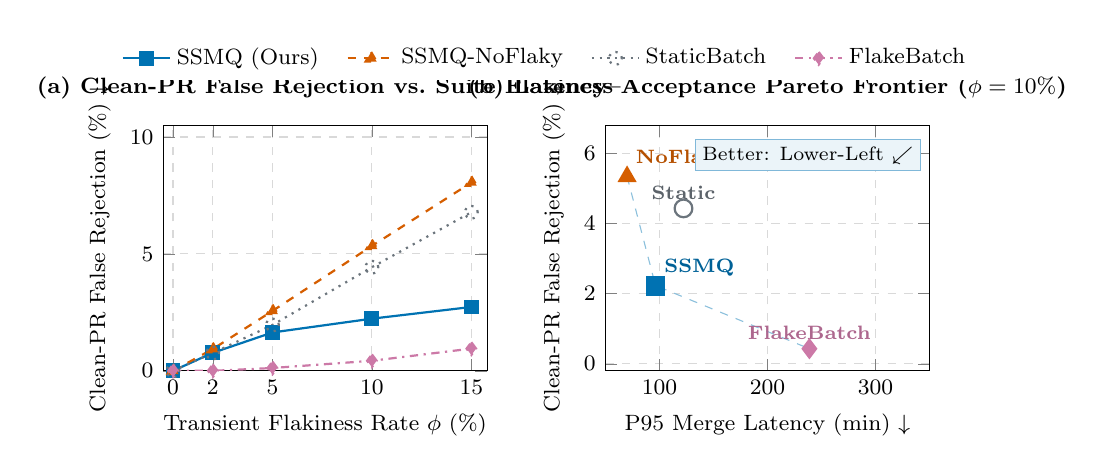
\begin{tikzpicture}
\begin{groupplot}[
  group style={group size=2 by 1, horizontal sep=1.5cm},
  width=0.47\textwidth, height=4.7cm,
  ymajorgrids=true, xmajorgrids=true, grid style={dashed,gray!30},
  tick label style={font=\footnotesize},
  label style={font=\footnotesize},
  title style={font=\footnotesize\bfseries},
  every axis plot/.append style={thick, mark size=2.3pt},
]
\nextgroupplot[title={(a) Clean-PR False Rejection vs.\ Suite Flakiness},
  xlabel={Transient Flakiness Rate $\phi$ (\%)}, ylabel={Clean-PR False Rejection (\%) $\downarrow$},
  xtick={0,2,5,10,15}, xmin=-0.5, xmax=15.8, ymin=0, ymax=10.5,
  legend to name=legFlaky, legend columns=4, legend style={font=\footnotesize, draw=none, /tikz/every even column/.style={column sep=8pt}}]
\addplot[color=ssmqBlue, mark=square*] coordinates { (0,0.00) (2,0.77) (5,1.64) (10,2.23) (15,2.73) }; \addlegendentry{SSMQ (Ours)}
\addplot[color=ssmqRed, mark=triangle*, dashed] coordinates { (0,0.00) (2,0.93) (5,2.56) (10,5.34) (15,8.05) }; \addlegendentry{SSMQ-NoFlaky}
\addplot[color=ssmqGray, mark=o, dotted] coordinates { (0,0.00) (2,0.76) (5,1.96) (10,4.43) (15,6.78) }; \addlegendentry{StaticBatch}
\addplot[color=ssmqPurple, mark=diamond*, dashdotted] coordinates { (0,0.00) (2,0.00) (5,0.12) (10,0.43) (15,0.95) }; \addlegendentry{FlakeBatch}
\nextgroupplot[title={(b) Latency--Acceptance Pareto Frontier ($\phi=10\%$)},
  xlabel={P95 Merge Latency (min) $\downarrow$}, ylabel={Clean-PR False Rejection (\%) $\downarrow$},
  xmin=50, xmax=350, ymin=-0.2, ymax=6.8]
\addplot[color=ssmqBlue!45, dashed, thin, forget plot] coordinates { (70.1,5.34) (96.4,2.23) (238.8,0.43) };
\addplot[only marks, color=ssmqRed, mark=triangle*, mark size=3.2pt] coordinates { (70.1,5.34) };
\node[font=\scriptsize\bfseries, anchor=south west, inner sep=3pt, text=ssmqRed!85!black] at (axis cs:70.1,5.34) {NoFlaky};
\addplot[only marks, color=ssmqBlue, mark=square*, mark size=3.2pt] coordinates { (96.4,2.23) };
\node[font=\scriptsize\bfseries, anchor=south west, inner sep=3pt, text=ssmqBlue!85!black] at (axis cs:96.4,2.23) {SSMQ};
\addplot[only marks, color=ssmqGray, mark=o, mark size=3.2pt] coordinates { (122.3,4.43) };
\node[font=\scriptsize\bfseries, anchor=south, inner sep=3pt, text=ssmqGray!85!black] at (axis cs:122.3,4.43) {Static};
\addplot[only marks, color=ssmqPurple, mark=diamond*, mark size=3.2pt] coordinates { (238.8,0.43) };
\node[font=\scriptsize\bfseries, anchor=south, inner sep=3pt, text=ssmqPurple!85!black] at (axis cs:238.8,0.43) {FlakeBatch};
\node[font=\scriptsize, anchor=north east, fill=ssmqBlue!8, draw=ssmqBlue!50, inner sep=2.5pt] at (axis cs:342,6.4) {Better: Lower-Left $\swarrow$};
\end{groupplot}
\node at ($(group c1r1.north)!0.5!(group c2r1.north)+(0,0.85cm)$) {\pgfplotslegendfromname{legFlaky}};
\end{tikzpicture}
\caption{Flakiness sensitivity ($\phi\in[0\%,15\%]$) and latency--acceptance Pareto frontier at $\phi=10\%$. Two-regime Beta-Binomial gating positions SSMQ on the Pareto knee, slashing clean-PR false rejections relative to \texttt{SSMQ-NoFlaky} and \texttt{StaticBatchBisect} while avoiding the tail-latency explosion of unconditional full-batch retries (\texttt{FlakeAwareBatch}).}
\label{fig:flaky_pareto}
\end{figure*}


\subsection{RQ5: Failure-Density Regime and Multi-Culprit Boundary of Blame}
Why does \texttt{ASTStackCausalRanker}---despite \BenchASTTopOnePct{}\% Top-1 accuracy on real Python failures---yield only a \RegimeNomBlameGainPct{}\% P95 reduction ($p\RegimeNomBlameP{}$) over binary bisection (\texttt{SSMQ-NoBlame}) at the default operating point? Table~\ref{tab:blame_regime} and Figure~\ref{fig:blame_regime}(b) test Proposition~\ref{prop:complexity} directly across four failure-density regimes (\texttt{v3\_exp8\_blame\_regime}):

% AUTO-GENERATED FROM v5_exp8_blame_regime — DO NOT EDIT
\begin{table}[t]
\centering
\footnotesize
\setlength{\tabcolsep}{2.3pt}
\caption{Controlled $2\times 2$ Factorial Blame Sweep ($\rho=80\%$ Fixed): Survivor P95 (min), Mean Failed-Root Size (FailSz), Share of All Failed Roots With $\ge 2$ Modeled Culprits (Multi\%), and 4-Cell Holm $p$ (SSMQ vs.\ NoBlame).}
\label{tab:blame_regime}
\begin{tabular}{lcccccc}
\toprule
\textbf{Cell ($q, K$)} & \textbf{Static} & \textbf{NoBlame} & \textbf{SSMQ} & \textbf{FailSz} & \textbf{Multi\%} & \textbf{Holm $p$} \\
\midrule
8\%, $K{=}8$ & 95.0 & 66.0 & \textbf{66.0} & 1.29 & 3.6\% & 1.0000 \\
16\%, $K{=}8$ & 102.6 & 56.5 & \textbf{56.5} & 1.25 & 3.8\% & 1.0000 \\
8\%, $K{=}12$ & 105.8 & 66.0 & \textbf{66.0} & 1.29 & 3.6\% & 1.0000 \\
16\%, $K{=}12$ & 114.9 & 56.5 & \textbf{56.5} & 1.25 & 3.8\% & 1.0000 \\
\bottomrule
\end{tabular}
\end{table}

% AUTO-GENERATED FROM v3_exp0_blame_microbench & v3_exp8_blame_regime — DO NOT EDIT
\begin{figure*}[t]
\centering
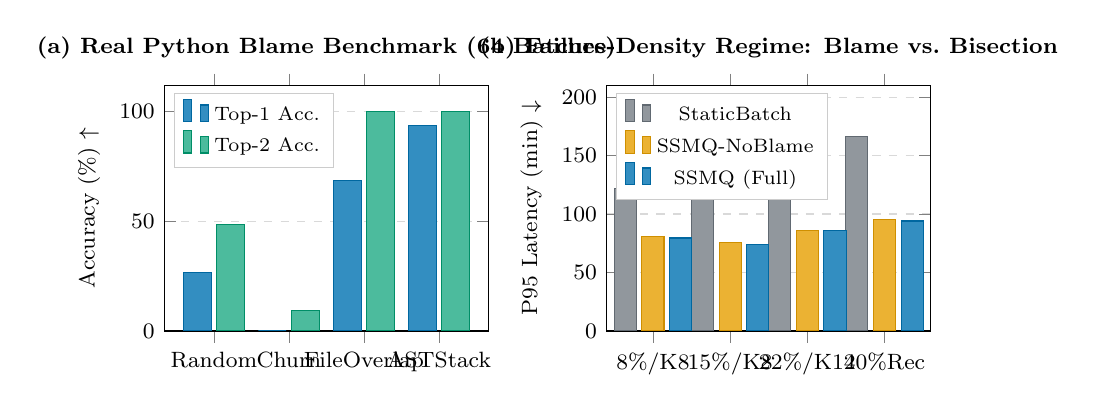
\begin{tikzpicture}
\begin{groupplot}[
  group style={group size=2 by 1, horizontal sep=1.5cm},
  width=0.47\textwidth, height=4.7cm,
  ymajorgrids=true, grid style={dashed,gray!30},
  tick label style={font=\footnotesize},
  label style={font=\footnotesize},
  title style={font=\footnotesize\bfseries},
]
\nextgroupplot[title={(a) Real Python Blame Benchmark (64 Batches)},
  ybar=2pt, /pgf/bar width=10pt, ymin=0, ymax=112,
  symbolic x coords={Random,Churn,FileOverlap,ASTStack},
  xtick=data, ylabel={Accuracy (\%) $\uparrow$}, enlarge x limits=0.22,
  legend style={at={(0.03,0.97)}, anchor=north west, font=\scriptsize, draw=gray!40}]
\addplot[fill=ssmqBlue!80, draw=ssmqBlue!90!black] coordinates { (Random,26.6) (Churn,0.0) (FileOverlap,68.8) (ASTStack,93.8) }; \addlegendentry{Top-1 Acc.}
\addplot[fill=ssmqTeal!70, draw=ssmqTeal!90!black] coordinates { (Random,48.4) (Churn,9.4) (FileOverlap,100.0) (ASTStack,100.0) }; \addlegendentry{Top-2 Acc.}
\nextgroupplot[title={(b) Failure-Density Regime: Blame vs.\ Bisection},
  ybar=2pt, /pgf/bar width=8pt, ymin=0, ymax=210,
  symbolic x coords={8\%/K8,15\%/K8,22\%/K12,40\%Rec},
  xtick=data, ylabel={P95 Latency (min) $\downarrow$}, enlarge x limits=0.20,
  legend style={at={(0.03,0.97)}, anchor=north west, font=\scriptsize, draw=gray!40}]
\addplot[fill=ssmqGray!75, draw=ssmqGray!90!black] coordinates { (8\%/K8,121.9) (15\%/K8,132.3) (22\%/K12,159.7) (40\%Rec,166.6) }; \addlegendentry{StaticBatch}
\addplot[fill=ssmqOrange!80, draw=ssmqOrange!90!black] coordinates { (8\%/K8,80.6) (15\%/K8,75.7) (22\%/K12,86.0) (40\%Rec,95.2) }; \addlegendentry{SSMQ-NoBlame}
\addplot[fill=ssmqBlue!80, draw=ssmqBlue!90!black] coordinates { (8\%/K8,79.5) (15\%/K8,73.8) (22\%/K12,85.6) (40\%Rec,94.0) }; \addlegendentry{SSMQ (Full)}
\end{groupplot}
\end{tikzpicture}
\caption{(a) Attribution accuracy across 64 real executed Python failing batches, demonstrating AST symbol-level + 1-hop call-graph gains over file-level traceback matching (\texttt{FileOverlap}). (b) Failure-density regime sweep contrasting \texttt{StaticBatch}, \texttt{SSMQ-NoBlame}, and full \texttt{SSMQ}: 1-step blame yields statistically significant P95 reductions in single-culprit regimes ($8\%$--$15\%$ defect, $K=8$) while saturating when high defect density ($22\%$, $K=12$) causes multi-culprit batches that fall back to bisection.}
\label{fig:blame_regime}
\end{figure*}


\begin{itemize}
    \item \textbf{Single-Culprit Sweet Spot ($q=8\%$--$15\%, K=8$)}: Because graph-disjoint packing already eliminates most on-graph conflicts and isolates high-risk PRs into protected lanes of size $K \le 2$ (where 1-step blame and binary split are identical), batch failures primarily occur when a single latent defect strikes a fast-lane batch. As individual defect rate increases from $8\%$ to $15\%$ at $K=8$, 1-step blame's end-to-end P95 advantage over \texttt{SSMQ-NoBlame} strengthens from -\RegimeNomBlameGainPct{}\% ($p\RegimeNomBlameP{}$) to -\RegimeElevBlameGainPct{}\% (\RegimeElevSSMQPNinetyFive{} vs.\ \RegimeElevNoBlamePNinetyFive{}~min, $p\RegimeElevBlameP{}$; and nearly $2\times$ faster than \texttt{StaticBatchBisect}'s \RegimeElevStaticPNinetyFive{}~min).
    \item \textbf{Multi-Culprit Saturation ($q=22\%, K=12$)}: Exactly as predicted by Proposition~\ref{prop:complexity}, when defect density climbs to $22\%$ with $K_{\max}=12$, the expected number of simultaneous culprits inside a failing fast-lane batch exceeds two. Evicting only Top-1 suspect $s_1$ leaves a second culprit in $B \setminus \{s_1\}$, triggering binary-bisection fallback and narrowing the P95 delta to -\RegimeHighDefBlameGainPct{}\% (\RegimeHighDefSSMQPNinetyFive{} vs.\ \RegimeHighDefNoBlamePNinetyFive{}~min, $p\RegimeHighDefBlameP{}$; recovery rounds \RegimeHighDefSSMQRounds{} vs.\ \RegimeHighDefNoBlameRounds{}). Across all regimes, however, SSMQ's combined architecture outperforms FIFO \texttt{StaticBatchBisect} by over $40\%$--$46\%$, and the blame accuracy sweep (\texttt{v3\_exp7\_blame\_sweep}, $50\%$--\BenchASTTopOnePct{}\%) confirms zero safety degradation under lower ranker precision.
\end{itemize}

\section{Related Work}
\label{sec:related}

We position SSMQ across four research areas and contrast its scheduling guarantees against prior merge-queue and CI optimization designs in Table~\ref{tab:related_taxonomy}.

\begin{table*}[t]
\centering
\footnotesize
\setlength{\tabcolsep}{7pt}
\caption{Qualitative Comparison of Merge Queue \& CI Verification Paradigms.}
\label{tab:related_taxonomy}
\begin{tabular}{lcccc}
\toprule
\textbf{System / Paradigm} & \textbf{Dependency-Aware} & \textbf{Speculation / Batching} & \textbf{Flaky Gating} & \textbf{Fault Attribution} \\
\midrule
Static Batching (Bors / GitHub~\cite{fallahzadeh2023accelerating}) & No (FIFO) & Static batch $K$ & None & $O(\log K)$ binary bisection \\
Linear Trains (GitLab Merge Trains) & No (FIFO) & Linear prefix train & None & Head abort \& restart \\
SubmitQueue (Uber~\cite{ananthanarayanan2019keeping}) & Risk model only & Pass/fail outcome tree & Implicit & Outcome-tree branch split \\
Flake-Aware Bisection~\cite{henderson2023flake} & No (FIFO) & Post-submit culprit search & Bayesian & Noisy binary bisection \\
Predictive Test Selection~\cite{machalica2019predictive,jin2023hybridcisave} & Test granularity & Single-PR build pruning & Orthogonal & N/A (composable) \\
\textbf{SSMQ (Ours)} & \textbf{Cone-Disjoint ($\hat{G}$)} & \textbf{Risk-Stratified Multi-Lane} & \textbf{2-Regime Beta-Binomial} & \textbf{1-Step AST/Stack + Fallback} \\
\bottomrule
\end{tabular}
\end{table*}

\textbf{CI Merge Queues, Batching, and Test Selection.}
Empirical studies of open-source and industrial repositories show that CI adoption improves defect containment and release cadence at the cost of queueing delay and compute contention~\cite{hilton2016usage,zhao2017impact,bernardo2023impact,wessel2023github}. At hyperscale, Google's TAP~\cite{elbaum2014techniques,memon2017taming} introduced batched regression testing, Uber's SubmitQueue~\cite{ananthanarayanan2019keeping} formulated speculative pass/fail outcome trees to sustain monorepo merge throughput, and Meta~\cite{juloori2025scale} decoupled pre-merge and post-merge verification into lean pipelines. Subsequent work investigated failure-history-guided dynamic batch sizing~\cite{bavand2021mining}, parallel batch testing with bisection~\cite{fallahzadeh2023accelerating}, risk-weighted commit bisection~\cite{najafi2019bisecting}, and queue reordering via PR prioritization~\cite{jungwirth2025improving}. A parallel line of work shrinks per-job execution time through test-selection policies based on state transitions~\cite{leong2019assessing}, predictive ML models~\cite{machalica2019predictive}, reinforcement learning~\cite{spieker2017reinforcement}, joint build-and-test filtering~\cite{jin2023hybridcisave}, and pipeline-aware scheduling~\cite{schwendner2025practical}. Whereas test selection prunes test suites \emph{within} a single build and prior batchers group PRs in arrival order, SSMQ intervenes at the \emph{batch formation} layer via warm-up cone disjointness---a mechanism orthogonal to, and directly composable with, per-batch regression test selection.

\textbf{Flaky Tests and Noisy Culprit Isolation.}
Field studies demonstrate that non-deterministic test failures permeate unit, UI, and integration suites~\cite{luo2014empirical,lam2020large,romano2021empirical,tahir2023test} and frequently cluster in correlated infrastructure bursts~\cite{parry2025systemic}. Program-analysis detectors such as DeFlaker~\cite{bell2018laker} and iDFlakies~\cite{lam2019idflakies} pinpoint flaky tests via differential coverage and test-order permutation. On the post-submit side, Ziftci and Reardon~\cite{ziftci2017broke} ranked suspect commits across failing Google builds, while Henderson et al.~\cite{henderson2023flake} formulated Bayesian noisy bisection under flaky outcomes. SSMQ embeds online conjugate Beta-Binomial flakiness estimation directly inside pre-merge queue scheduling and introduces asymmetric thresholds for singletons versus multi-PR batches to balance tail latency against clean-PR false rejections.

\textbf{Semantic Merge Conflicts and Change Impact Analysis.}
Prior work has predicted textual and build conflicts from historical edit patterns~\cite{owhadikareshk2019predicting}, applied PR-level change impact analysis to guide reviewer assignment~\cite{gmen2025enhanced}, and trained neural transformers and language models to synthesize merge resolutions after conflicts surface~\cite{zhang2022trained,svyatkovskiy2022program}. Rather than repairing broken merges post hoc, SSMQ leverages leak-free co-change and directory cones to prevent potentially interfering PRs from co-habiting fast-lane batches while automatically re-verifying isolated PRs when latent interactions occur.

\textbf{Fault Localization and Traceback Attribution.}
Spectrum-based fault localization (SBFL) methods such as Tarantula~\cite{jones2005empirical} and Ochiai~\cite{abreu2009practical} compute statement suspiciousness from per-test coverage matrices, whereas recent approaches fine-tune large language models on mutation-generated stack traces~\cite{jambigi2025fault}. Recording fine-grained coverage matrices on every CI run or invoking multi-second LLM inference inside the scheduler control loop imposes nontrivial operational overhead. SSMQ's \texttt{ASTStackCausalRanker} instead combines zero-instrumentation AST function diffs with 1-hop stack-trace call-graph reachability, isolating suspect PRs in \BenchASTMs{}~ms with fail-safe bisection fallback.

\section{Discussion, Deployment Guidance, and Threats to Validity}
\label{sec:threats}

\subsection{Practical Deployment Blueprint for High-Velocity CI}
Our experimental findings distill into four engineering guidelines for teams operating GitHub Merge Queue, GitLab Merge Trains, Bors, or Zuul at high merge velocity:
\begin{enumerate}
    \item \textbf{Prioritize Dependency-Disjoint Packing Over Deeper Speculation}: Even a faithful EuroSys~'19 outcome-tree SubmitQueue~\cite{ananthanarayanan2019keeping} incurs a \UberInvalidRatePct{}\% speculative invalidation rate when arrival-ordered batches combine overlapping module edits. Mining a warm-up co-change and two-level directory graph requires zero build-system instrumentation, executes in under a millisecond per dispatch, and preserves large P95 latency and compute reductions even when $60\%$ of semantic conflicts lie off-graph ($\rho=40\%$).
    \item \textbf{Guard Singletons---Not Multi-PR Batches---Aggressively Against Flakes}: Benchmarking merge queues purely on merged-PR latency conceals false rejections of clean patches. Enforcing asymmetric posterior thresholds ($\tau_1 = 0.25$ before rejecting singletons vs.\ $\tau_B = 0.50$ before rerunning multi-PR batches) eliminates most flaky rejections without incurring the tail-latency blowup of unconditional batch retries.
    \item \textbf{Deploy Static AST/Traceback Blame as a Sub-3~ms First Filter}: On our \BenchTotalBatches{}-batch executed benchmark, AST function-diff filtering eliminates co-file comment and documentation distractors (\BenchASTCofilePct{}\% vs.\ \BenchFileCofilePct{}\% Top-1 for file-level overlap) in \BenchASTMs{}~ms. Production pipelines should run deterministic AST/traceback ranking as an immediate first stage, invoking heavier LLM-based fault localization~\cite{jambigi2025fault} only when multi-culprit or cross-service failures defeat static reachability.
    \item \textbf{Adaptively Evict Top-$k$ Suspects Under High Failure Density}: As established in RQ5, single-suspect eviction ($k=1$) saturates when batch defect density reaches $22\%$ at $K=12$ because failing batches routinely harbor multiple culprits. Extending Algorithm~\ref{alg:blame} to evict Top-$k$ suspects whenever $\text{score}(s_2) / \text{score}(s_1) > 0.8$---or dynamically tightening $K_{\max}$ as observed failure rates climb---directly addresses noisy integration branches.
\end{enumerate}

\subsection{Threats to Validity}
\textbf{Construct Validity.} Although file-touch topologies, hotspot skew, and inter-arrival gaps come directly from 600 chronologically merged GitHub PRs, the GitHub GraphQL API truncates per-PR file lists beyond $40$ paths, and public merge histories do not record pre-merge queue rejections or exact enqueue timestamps. Moreover, while our v3 simulator decouples the ground-truth conflict oracle $G^*$ from $\hat{G}$ via latent off-graph interactions, includes a zero-conflict control ($P_c = 0$), and enforces cumulative mainline verification for persistent conflicts, per-PR defect probabilities and pairwise conflict densities remain parameterized rather than replayed from proprietary corporate CI failure logs. Finally, our executable blame benchmark evaluates \BenchTotalBatches{} real failing batches in a six-module Python repository; polyglot monorepos featuring asynchronous RPCs, C++ templates, or Go goroutine crash dumps may yield lower static Top-1 precision---a degradation that SSMQ absorbs safely via deterministic bisection fallback across our $50\%$--\BenchASTTopOnePct{}\% ranker-accuracy sweep.

\textbf{Internal and Conclusion Validity.} Sharing matched $(\text{repo}, \text{seed})$ defect and conflict realizations across all schedulers, calibrating 20-seed A/A noise floors, and reporting $95\%$ bootstrap confidence intervals alongside Holm-Bonferroni-corrected paired Wilcoxon tests and Cliff's $|\delta|$ effect sizes mitigate stochastic variance and family-wise Type-I error. Because each replay drains a finite 150-PR evaluation stream per repository rather than an infinite-horizon stationary process, reported P95 latencies reflect finite-burst drain behavior rather than asymptotic queueing equilibrium.

\textbf{External Validity.} Organizations employing fine-grained build caching (where small diffs verify an order of magnitude faster than core edits) or multi-hour hardware-in-the-loop suites may need to retune $K_{\max}$, $\theta_{\text{risk}}$, and $(\tau_1, \tau_B)$. Likewise, extending \texttt{ASTStackCausalRanker} beyond Python to TypeScript, Go, or Rust monorepos requires language-agnostic syntax trees such as Tree-sitter. Shadow-deploying SSMQ alongside GitHub Merge Queue on an active open-source monorepo represents our primary avenue for production validation.

\section{Conclusion}
\label{sec:conclusion}

We presented \textbf{SSMQ}, unifying leak-free warm-up cone-disjoint packing, two-regime Beta-Binomial flaky gating, and fail-safe 1-step AST/traceback suspect ranking. On \BenchTotalBatches{} counterbalanced Python failure batches, \texttt{ASTStackCausalRanker} reaches \BenchASTTopOnePct{}\% Top-1 accuracy and \BenchASTLOOPct{}\% LOO recovery in \BenchASTMs{}~ms (\BenchASTMaxMs{}~ms max), outperforming a nested file ablation on 50/50 sibling edits (\BenchASTSiblingPct{}\% vs.\ \BenchFileTriviaSiblingPct{}\%). Across 10 exact-Git-tree replays, SSMQ cuts live CI runs by \GitReplayCISavePct{}\% and bisection splits by \GitReplaySplitSavePct{}\% (\TotalEscapedDefects{} escapes). Across \TotalSealedRuns{} sealed v5 suites (\TotalSealedRecords{} replay records, \TotalEscapedDefects{} modeled escapes), SSMQ lowers survivor P95 latency by \LatRedVsStaticPct{}\% vs.\ static FIFO ($p\HolmPLatVsStatic{}$) and \LatRedVsDepTreePct{}\% vs.\ bridge-safe dependency-aware outcome trees ($p\HolmPLatVsDepTree{}$), holding under uncorrelated defects and reversing cleanly at $0\%$ recall and zero conflict.

\section*{Data Availability}
A blinded replication package containing the Python standard-library simulator, \BenchTotalBatches{}-batch executable benchmark, real-Git queue executor, auditable GitHub trace fetcher (\texttt{scripts/fetch\_traces.py}), 600-PR consecutive traces with \texttt{fetch\_manifest.json}, all \TotalSealedRuns{} SHA-256-sealed v5 runs, 25 unit tests, and deterministic verification script (\texttt{python3 eval/audit.py --verify-only}) is archived for anonymous review and will be publicly released upon acceptance.

\section*{AI-Assisted Tooling Disclosure}
The authors used Codex and Antigravity models for literature discovery, implementation, analysis, manuscript drafting, and simulated peer review. The artifact identifies the executable inputs and outputs behind the empirical results. Model reviews are internal editorial checks. The authors are responsible for the final claims and submission.


\bibliographystyle{IEEEtran}
\bibliography{refs}

\end{document}
